% SPDX-License-Identifier: CC-BY-4.0
% 中文镜像稿 v0.3.2(2026-10-21),与 main.tex 逐段对齐;数字由 tools/check_numbers.py --tex main_zh.tex 对账。
\documentclass[11pt,a4paper]{ctexart}
\usepackage[margin=2.5cm]{geometry}
\usepackage{amsmath,amssymb}
\usepackage{booktabs}
\usepackage{graphicx}
\usepackage{xcolor}
\usepackage{pgfplots}
\pgfplotsset{compat=1.18}
\usepackage[numbers,sort&compress]{natbib}
\usepackage[hidelinks]{hyperref}
\usepackage{enumitem}
\usepackage{caption}
\captionsetup{font=small,labelfont=bf,justification=raggedright,singlelinecheck=false}
\graphicspath{{figures/}}
\newcommand{\hashtrunc}[2]{\texttt{#1\ldots#2}}
\newcommand{\um}{µm}
\newcommand{\tox}{TX100}
\title{机器学习液滴微流控设计代理模型的可靠性审计:\\一次密封的负面验证、偏移诊断与物理引导的硬约束}
\author{Zhiyuan Zhang\thanks{独立研究。通讯方式见公开仓库 \url{https://github.com/LibertychaserUS/microfluidic-native-physics}。稿件正文与原创图件以 CC~BY~4.0 发布,代码以 Apache-2.0 发布。本工作尚未分配 arXiv 标识符或 DOI。本文为英文稿 main.tex 的中文镜像,内容逐段对齐;如有歧义,以英文稿为准。}}
\date{草稿 v0.3.2 —— 2026 年 10 月 21 日}

\begin{document}
\maketitle

\begin{abstract}

机器学习代理模型日益被用于指导液滴微流控设计,但其可靠性通常只在随机训练/测试划分上报告。我们基于公开表格数据开展了一次回顾性可靠性审计。在复现一个已发表的流动聚焦基线时,随机划分下的直径误差(5.27\% MAPE)在外部文献来源上约翻一倍(10.97\%),名义 90\% 的共形区间仅覆盖 55.1\% 的外部行,无标签适用域剪枝把 10 µm 成功率从全部外部候选的 59.4\% 提高到保留候选的 92.3\%,同时保留了全部成功候选的 63.2\%——一项考虑依赖结构的重新分析把这一增益归因于哪些文献来源被保留,而非来源内部的区分能力。两次预注册的密封验证都得到负面结果:一个冻结模型对整个留出的表面活性剂化学体系(87 行)的预测 MAPE 为 19.84\%、覆盖率 44.8\%,尽管每一行都位于边际训练范围之内;另一个冻结模型对一个独立实验室的脂质体尺寸(57 行)的预测 MAPE 为 240.39\%,并在 38.6\% 的行上给出负直径;对同一配置在尺寸对数上做事后重拟合消除了负预测,但误差仍约为其自身开发参照的两倍半。一个在拟合前冻结的、带硬结构约束的物理引导回归器——而非经典 PINN——相对于已发表的基线并未降低化学体系宏平均误差,尽管其边界消除了物理上无效的预测。一个覆盖两个数据集上七个偏移单元的方法矩阵,并扩展到三类不确定性感知模型族与协变量偏移加权的共形区间,表明单乳液与双乳液之间的器件类型偏移是这些数据中最大的偏移(相对随机划分参照的误差比为 3.30 和 10.31),并且当训练支撑与测试支撑不重叠时,没有任何模型族或重加权能恢复区间覆盖率。据我们所知,此前尚无经同行评审的、针对微流控设计代理模型的密封预测审计;检索依据已记录在案。所有分析均为基于公开数据的回顾性分析;未进行也未声称任何湿实验验证。

\end{abstract}

\section{引言}
\label{sec:intro}

液滴微流控中的自动化实验面临一个组合式的设计空间:通道几何、流速、流体性质与表面活性剂化学相互作用,共同决定液滴尺寸与生成速率。在公开实验表格上训练的机器学习(ML)代理模型,如今已被用于在该空间中导航 ~\cite{lashkaripour2021,lashkaripour2024,samari2025}。然而,它们所报告的精度几乎总是来自随机的行级训练/测试划分,而这并不代表代理模型的实际部署方式:使用者会把它应用到一种新器件、一种新流体对,或一种训练表中从未出现过的新表面活性剂上。

我们对 DAFD 3.0 基线 ~\cite{lashkaripour2024} 的独立复现给出了两个数字,它们构成了本文的动机。在 868 行综合表的 15 次随机 80/20 划分上,已发表的 XGBoost 配置达到的直径 MAPE 为 $5.268\% \pm 0.421\%$;在同一论文发布的 64 行外部文献集上,误差为 $10.971\% \pm 0.552\%$——大约翻了一倍。在随机划分上校准的名义 90\% 共形化分位数回归区间,覆盖了 91.03\% 的内部测试行,但只覆盖 55.10\% 的外部行。

本文并非再提出一种逆向设计算法或一种通用的物理信息架构,而是对微流控 ML 设计代理模型在部署偏移下做一次系统的可靠性审计,并给出该审计所产生的证据;本文不就硬约束与软约束孰优孰劣作一般性论断。这些证据专属于液滴微流控代理模型,并且若无密封测试便不可能获得:一是在未见过的表面活性剂化学体系上发生的失效,而此时每个留出行都落在边际训练范围之内,因此边际适用性筛选对此毫无察觉;二是对无标签剪枝在文献数据上究竟带来什么的量化说明——这是一种来源层面的增益,而一个水力直径代理指标即可与之持平;三是对带硬结构边界的物理引导是否会改变上述任何结果的冻结检验;四是覆盖两个公开数据集上七个偏移单元的方法矩阵基准;五是在一个独立公开数据集上、于实验室偏移条件下进行的第二次密封验证。本文共同报告六个组成部分:

\begin{enumerate}[leftmargin=*,itemsep=2pt]
\item \textbf{分布偏移基准。} 我们复现 DAFD 3.0 基线,并量化从随机划分到分组划分、再到外部文献来源的性能退化,包括共形覆盖率的丧失(第~\ref{sec:r1}–\ref{sec:r3}、\ref{sec:r7}~节)。
\item \textbf{一次密封的负面验证(V1)。} 我们在看到任何标签之前,将公开的 Chagot 等 ~\cite{chagot2022} 数据集中完整的 Triton X-100(TX100)表面活性剂组密封起来,冻结了模型、终点和决策判据,并且只揭示一次标签。结果为负面,并连同揭示过程的完整记录一并保留(第~\ref{sec:v1protocol}、\ref{sec:incident}、\ref{sec:r5}~节)。
\item \textbf{对无标签剪枝的精确率—召回率分析。} 仅由训练输入构建的适用性筛选提高了保留候选的成功率,但同时丢弃了成功的候选;我们连同各自的分母一并报告这两个数字,并给出负对照,表明该增益是来源层面的而非候选层面的(第~\ref{sec:r4}、\ref{sec:r7}~节)。
\item \textbf{一个经过审计的设计侧对象(V2)。} 一个基于原生变量、带硬结构约束的物理引导回归器——而非经典 PINN——在拟合之前按其自身方案冻结,并且仅在 TX100 揭示之后做回顾性评估。其锁定的决策规则给出负面/混合的结论:相对于采用已发表特征的基线,它并未降低化学体系宏平均误差,而其硬输出边界消除了物理上无效的点预测(第~\ref{sec:v2protocol}、\ref{sec:r6}~节)。
\item \textbf{跨偏移类型的方法矩阵基准。} 在其自身的冻结方案下,三种点预测模型、四种区间估计器和五种适用性评分(外加随机与仅尺寸对照)被运行于跨越两个数据集的七个偏移单元——随机参照、器件几何、跨文献、单乳液到双乳液与双乳液到单乳液、整体化学体系留一——共两次独立运行,产物清单哈希逐字节一致;另有两个冻结方案在相同单元上重跑,分别针对三类具备不确定性感知的模型族和协变量偏移加权的共形区间(第~\ref{sec:w3protocol}、\ref{sec:w4protocol}、\ref{sec:w5protocol}、\ref{sec:r8}~节)。
\item \textbf{在独立数据集上的第二次密封验证。} 密封预测协议在下载之前第二次被实例化,对象是一个公开的跨实验室脂质体数据集,整个第二个实验室被密封;结果为负面,并连同完整的时间线一并保留(第~\ref{sec:d3protocol}、\ref{sec:r9}~节)。
\end{enumerate}

第~\ref{sec:outlook}~节陈述的是一份计划而非结果,即这些失效模式对于收集数据、构建能在更大器件和新材料上保持精度的代理模型意味着什么。

我们提出两项刻意受到限定的论断,每一项都以附录~\ref{app:search}中的检索依据为限定。第一,据我们所知,尚无经同行评审的工作将密封预测可靠性审计应用于微流控 ML 设计代理模型;本文在两个独立的公开数据集上报告了两次此类审计。第二,据我们所知,尚无经同行评审的工作在微流控领域把物理引导、架构层面的硬约束与逆向设计评估统一于单一框架;最接近的工作是用于确定性侧向位移(deterministic lateral displacement,DLD)设计的周期性强制网络 ~\cite{lee2025},以及一种优化层的修复算子 ~\cite{micromixer2026},它们与我们的区别在于各组件的组合方式,而非种类上的不同。我们并不声称自己是第一个微流控逆向设计或 ML 系统,是第一个物理引导的微流控模型,也不是第一个发表负面结果的工作。

\paragraph{预先声明的假设} 2026 年 7 月 16 日的项目记录在扩展分析实施之前固定了四条可证伪的假设(此处译自原始记录,措辞未作其他改动):

\begin{description}[leftmargin=*,itemsep=1pt]
\item[H1] 在跨文献、跨器件和跨流体条件下,随机 80/20 划分会高估模型的可靠性。
\item[H2] 在分布内随机划分上达到名义覆盖率的不确定性区间,在独立文献偏移下会显著丧失覆盖率。
\item[H3] 仅由训练输入分布构建的无标签适用域,能够识别出一部分高风险的外部候选,并提高满足直径容差的保留候选所占的比例。
\item[H4] 将液滴直径模型与体积守恒关系耦合,可把几何搜索与流速搜索统一为工程上可执行的直径—频率目标。
\end{description}

H1–H3 被直接评估;H4 仅在质量守恒频率复现的层面上得到处理(第~\ref{sec:r1}~节),其余部分则留待未决。

\section{相关工作}
\label{sec:related}

\paragraph{用于液滴与器件设计的 ML} 流动聚焦液滴发生器的设计自动化,已从 DAFD 1.0 ~\cite{lashkaripour2021},经由通用性/稳定性优化 ~\cite{mcintyre2023},发展到 DAFD 3.0 的单乳液与双乳液预测器,后者配有约束搜索并报告了湿实验测试 ~\cite{lashkaripour2024}。以仿真训练的代理模型(DesignFlow~\cite{samari2025})、确定性侧向位移设计网络 ~\cite{vatandoust2022}、模块化芯片架构设计 ~\cite{li2026pathchip}、ML 自动化的微流控回路设计 ~\cite{mufg2026} 以及流动编程网络 ~\cite{ceyehao2026},则覆盖了跨器件类别的逆向设计。我们把这批文献视为审计的对象,而不是有待填补的空白。

\paragraph{物理引导建模与硬约束} 物理引导的微流控模型大多把物理以软惩罚项的形式施加,或采用评估微分方程残差的物理信息神经网络(physics-informed neural network,PINN) ~\cite{bpgnn2026,flexpinn2026,raissi2019};一项针对电磁微混合器的、经贝叶斯优化的物理引导网络,明确把"不求解完整 Navier–Stokes 方程而高效嵌入宏观约束"列为未解决的问题 ~\cite{bpgnn2026}。架构层面的硬约束出现在用于 DLD 器件的周期性强制网络中 ~\cite{lee2025},而带修复算子的约束感知优化则出现在自主微混合器设计中 ~\cite{micromixer2026}。硬约束是一个有别于 PINN 惩罚项的概念,并且在外推条件下可优于软惩罚,这在一般场景中已有确立 ~\cite{naturecs2021,baty2023,prnet2026};我们不再重新讨论。一项物理约束的沸腾代理模型报告称,约束在训练包络之内有帮助、在其之外则有损害 ~\cite{filmpinn2026},这正是我们的审计针对一个微流控对象所量化的那种依赖于工况的问题。因此,下文的 V2 模型被称为带硬结构约束的物理引导回归器,而不是经典 PINN:公开表格中不含速度场或压力场、界面坐标、时间坐标或边界条件观测值,因而没有可供评估偏微分方程残差的位置。

\paragraph{无量纲学习与原生变量} 有相当多的工作把量纲不变性嵌入学习之中,从稀缺数据中发现支配性的无量纲数群 ~\cite{xie2022,oppenheimer2023};一项近期的液滴研究把量纲分析与学习结合起来,报告其在训练器件中未见过的黏度曲线上 $R^2$ 为 0.80–0.83,而对强剪切稀化流体为 0.46,对新的通道深度为 0.48 ~\cite{labchip2025dimless}——这是流变学与器件偏移下的退化,而不是外推本身的失败。我们并不声称在原生记录变量上建模是新的或更好的;大多数表格式微流控 ML 本来就是在原始量上运作的。我们的立场是一种*接口纪律*(interface discipline):V2 只信任原生记录的量(流速、平衡界面张力、浓度、临界胶束浓度(critical micelle concentration,CMC)、无表面活性剂指示变量),并根据固定的单位和器件常数以确定性方式重新计算流速比、毛细数和雷诺数;调用方不能独立地提供任何无量纲数。我们提供的唯一比较性证据,是在一个方案、一个划分下做的消融:原生输入的 XGBoost 基线(B2)的化学体系宏平均 MAPE 为 9.13\%,而已发表的四输入基线(B1)为 10.27\%(第~\ref{sec:r6}~节)。这是一个方案内的消融,并非关于原生变量在化学体系偏移下可靠性的结论,也不是 V2 的属性,因为 V2 并没有胜过 B1。

\paragraph{可靠性审计、预注册与负面结果} 训练之后对逐点可靠性做审计,由 Schulam 和 Saria ~\cite{schulam2019} 提出了框架;预测建模的预注册已被提议用于 ML ~\cite{hofman2023};发表负面结果是一种已确立的做法,有其专门的发表渠道和近期的一篇立场论文 ~\cite{karl2024};数据泄漏是公认的导致结论被夸大的因素 ~\cite{kapoor2023}。共形预测在可交换性条件下给出有限样本的边际覆盖率 ~\cite{romano2019},而协变量偏移下的覆盖率则需要额外的结构,例如已知或估计的密度比 ~\cite{tibshirani2019};对于留出化学体系的迁移,我们两者都不主张。针对力学主导流动中物理信息代理模型的训练前可辨识性审计 ~\cite{cieslak2026},是微流控之外在方法上最接近的相关工作。在微流控内部,综述把缺乏标准化基准、跨实验室泛化以及显式的外部验证列为未决问题 ~\cite{labchip2025review,das2025,delgiudice2026},而一个经过整理的跨实验室脂质体数据集则解决了数据层的问题 ~\cite{smartmicrofluidics2026};我们没有发现任何在微流控设计代理模型上实施密封预测审计的实例(附录~\ref{app:search})。

\paragraph{与 Vepa (2026) 的关系} 与我们最接近的是 Vepa ~\cite{vepa2026},其对机器学习的钠阴极电压相对于以实验为锚点的文献值做了预注册验证,并报告了其失败。我们与其共享预注册的精神,但在以下方面有所不同:领域(液滴微流控,而非材料信息学);被审计的对象(一个冻结的、物理引导且带硬约束的设计代理模型,与采用已发表特征的基线并列评估);以及搜索空间终点(无标签剪枝的精确率与召回率,以及回顾性的目标检索覆盖率)。Vepa 预注册了一项后续的校准审计,而我们则声明:任何针对 V2 的新的盲测论断都需要一个不同的、从未被检视过的数据集;我们也确实进行了一次这样的进一步密封测试——针对采用已发表特征的基线,在第三个数据集上——其负面结果见第~\ref{sec:r9}~节。

\section{数据与来源}
\label{sec:data}

本文使用三个公开数据集,全文称为 D1、D2 和 D3。D1 和 D2 承担液滴直径审计;D3 仅用于第二次密封验证,绝不与它们合并。

\paragraph{D1:DAFD 3.0(OSF 938rs)} 综合表有 868 行,外部泛化表有 64 行,来自四个文献来源(Galogahi 等,$n=24$;Lashkaripour 等,$n=20$;Roumpea 等,$n=14$;Mazutis 等,$n=6$)~\cite{lashkaripour2024}。使用八个已发表的输入:孔口宽度、黏度比、毛细数、流速比,以及四个归一化的几何描述符;目标为液滴直径。868 行中包含 474 个单乳液行,以及由成对的内/外相行(394 行)表示的 197 个双乳液工况;外部 64 行中包含 44 个单乳液行和 10 个双乳液工况(20 行)。所下载的四个工作簿的 SHA-256 摘要列于附录~\ref{app:hashes}。OSF 存储库的内容不做再分发;其对象级的再分发条款仍有待核实,方可建立任何镜像。

\paragraph{D2:Chagot 等(Zenodo 7055018,CC BY 4.0)} 两个 MATLAB 表(392 行和 76 行)给出了在一个固定的椭圆形流动聚焦结点(195 µm $\times$ 190 µm)上的 468 个配置,其输入为连续相与分散相流速、平衡界面张力、表面活性剂浓度和临界胶束浓度(CMC),输出为液滴直径(mm) ~\cite{chagot2022}。化学体系组仅由所记录的 CMC 值定义。行数账目如下。完整的 TX100 组(CMC $=3.5$ mM,87 行)是密封留出集,因此 V1 开发集为其余 $468-87=381$ 行;其中包含两行 CMC $=0.60$ mM 的数据(该值并未列在该论文的表面活性剂之中),因为 V1 密封时尚无任何隔离规则。此后的每一项分析(V2 与方法矩阵)都隔离这两行且从不重新归组,剩下六组共 466 行(CMC 为 0、2、3.5、4.33、11 和 20 mM,分别有 63、30、87、15、178 和 93 行),其中五个非 TX100 组共 379 行。

\paragraph{D3:Smart Microfluidics 脂质体数据集(Zenodo 17867478,CC BY 4.0)} 仅用于第二次密封验证(第~\ref{sec:d3protocol}~节)。该记录记载了在微混合器芯片上生产微流控脂质体的过程:输入为四种脂质组分(ESM、HSPC、CHOL、DSPE-PEG2000;mg/mL)、总流速(mL/min)、流速比和水相介质(MQ 或 PBS),输出为脂质体尺寸(nm)、多分散指数和一个成形标志 ~\cite{smartmicrofluidics2026}。作者发布的清洗后表格不含实验室字段,因此我们转而绑定作者经检查程序处理的原始文件:实验室 A(Latina,操作者 A,设备 A)提供开发集,在隔离 Droplet-chip 行以及输入或尺寸缺失的行之后共 246 行;实验室 B(Rome,操作者 A,等效设备 B)提供密封集,共 57 行。来自实验室 A 的一个 12 行的操作者 B 集合被作为次级集密封,不属于主要估计目标(estimand)。其目标与 D1 和 D2 不同(脂质体尺寸而非液滴直径),这是 D3 结果与它们分开报告的原因之一。

\paragraph{许可边界} 稿件正文和原创图件为 CC BY 4.0,代码为 Apache-2.0;二者均不对源论文或数据集重新授权。发布树中不包含任何第三方原始数据。

\section{方法}
\label{sec:methods}

\subsection{基线复现(E0)}
\label{sec:e0}

我们依据 ~\cite{lashkaripour2024} 中所述的方法参数重新实现了已发表的 XGBoost 配置,未复制上游代码(100 棵树,平方误差,学习率 0.3,最大深度 6,L2 正则化 1,最小子节点权重 1),并在 868 行表上重复了 15 次随机 80/20 划分。生成频率由质量守恒推出,$F = 6Q_d/(\pi d^3)$,并与已发表的频率误差比较。外部评估使用全部 868 行训练,并预测 64 个外部行。冻结的库版本已记录在案(XGBoost 3.3.0、scikit-learn 1.9.0、Python 3.12.13)。

\subsection{DAFD 上的扩展回顾性方案}
\label{sec:expanded}

由于 64 行外部集在先导阶段已被检视过,扩展的 DAFD 分析是回顾性和探索性的;一份冻结方案在实施之前固定了每一种方法、阈值、终点和负对照,从而使事后无法做出由结果驱动的改动。评估方案包括:15 次行随机划分(仅用于复现);15 次按精确输入分组的划分(exact-input grouped splits);30 次按器件几何分组的划分;30 次按几何加黏度比分组的划分(即“几何加流体”分组);以及全量训练后在固定外部集上测试。分组标识符是分组关系与双乳液内/外相配对链接的连通分量,因此一个配对绝不会跨越拟合/测试边界。模型为已发表的 XGBoost 配置(主模型)、随机森林和直方图梯度提升(仅作稳健性检验)。区间比较的是分裂共形(split conformal)、共形化分位数回归(conformalised quantile regression,CQR)和归一化分裂共形,在行随机和几何分组两种方案下均不使用外部标签进行校准;分组校准按依赖组内的最大值聚合非一致性得分。适用性评分包括:逐特征 min–max、标准化的 $k$ 近邻距离($k\in\{3,5,10,20\}$)、OAS 收缩 Mahalanobis 距离、Isolation Forest、局部离群因子(Local Outlier Factor)、单类 SVM、自助法集成分歧,以及一个袋外(out-of-fold)残差风险模型;阈值取留出校准得分的 0.90/0.95/0.975/0.99 分位数,并以连续的风险—覆盖曲线为主要对象,用对并列值不变(tie-invariant)的风险—覆盖曲线下面积(area under the risk–coverage curve,AURC)来概括。必须设置的负对照包括:在匹配预算下的随机评分与随机保留、来源内与来源内情境物理聚类的置换、仅水力直径与仅预测尺寸的评分,以及标签打乱的预测器。回顾性目标搜索重放为每个外部来源使用单独的候选池,采用 30–230 µm 的固定目标网格,在排序阶段隐藏结果,并且只报告已作答查询中的精确率,同时报告查询覆盖率和成功目标的召回率。Benjamini–Hochberg(BH)校正在每个检验族内部施行。

\subsection{密封化学留出(V1)}
\label{sec:v1protocol}

V1 方案在两个 MATLAB 文件被下载或打开之前就已写成并做了哈希(锁定时间 2026-07-16T12:27:58Z)。一个保管人程序按已发表的 TX100 CMC 值对合并后的 468 行进行了划分,写出一份带标签的 381 行开发表、一份仅含输入的 87 行盲测表,以及一份单独密封的标签文件(仅属主可读),并且只打印计数和哈希。点预测模型复现了源论文的 XGBoost 设置(100 个估计器,深度 3,学习率 0.3,种子 42),基于四个已发表的输入,在开发集上只拟合一次,不做任何基于盲测标签的调参。一个 90\% 的分裂共形区间在开发集的化学体系组上做了校准。四种适用性筛选(严格 min–max、取开发集第 95 百分位的 5-NN、OAS Mahalanobis、Isolation Forest)和针对 13 个固定目标(0.06–0.18 mm)的六种目标搜索策略均被冻结。预先声明的终点是:盲测 MAPE 对照一个复现判据($<11.4\%$,即已发表的半经验基准)和一个强复现判据($\le 6.0\%$),另加四个条件,在这些条件下方可称某条适用性规则为有益。完整的揭示前预测包(87 个预测、78 个查询—策略对、240 个排序候选)在一次性揭示闸门被消耗之前已做了哈希(摘要见附录~\ref{app:hashes})。这两个阈值的来源值得说明一下。11.4\% 这一数字,是源论文基于物理的基准——第~\ref{sec:v2protocol}~节所述的 Kalli 等关联式——在源论文随机的 76 行测试划分上的误差;6.0\% 则是围绕源论文 3.9\% 的随机划分 XGBoost 结果 ~\cite{chagot2022} 所设的容差。因此二者都锚定于分布内性能,而本文论证这会高估偏移下的可靠性;至于后来用于 D3 那种风格的、开发侧的留一化学体系(leave-one-chemistry-out)参照,并未在 V1 中预先注册,而是回顾性计算的(第~\ref{sec:posthoc}、\ref{sec:r5}~节)。

\subsection{揭示事故与仅涉及序列化的恢复}
\label{sec:incident}

揭示闸门在 2026-07-16T12:30:53Z 被消耗。程序核验了所有冻结的哈希,通过不透明的行标识符把预测与标签连接起来,计算了每一个锁定的终点,随后在最后一步写入时失败,原因是未作答的目标搜索查询带有 IEEE \texttt{NaN} 字段,而严格的 JSON 写入器正确地拒绝了它们。预期的结果文件从未被创建。一个单独的恢复程序——它在不修改冻结的揭示实现(摘要见附录~\ref{app:hashes})的情况下被加入——重新验证了所有哈希,重新核验了不透明 ID 集合的精确相等,基于已经解封的标签重新计算了同样的锁定指标,并且仅把未定义的 \texttt{NaN} 查询字段转换为 JSON \texttt{null}。恢复于 2026-07-16T12:32:58Z 完成;恢复得到的结果文件的摘要列于附录~\ref{app:hashes}。没有任何模型被重新拟合,没有任何排序被重新计算,没有任何指标被重新定义,也没有任何揭示前的产物被修改。因此,就所有预测、掩码、排序和决策规则而言,该验证仍然是前瞻性的,但我们将其描述为一次密封预测加一次已披露的仅涉及序列化的恢复,而不是一次在操作上毫无瑕疵的一次性揭示。一份事后复盘把根本原因追溯到 Python 宽松的 \texttt{allow\_nan=True} 默认值,以及缺少单一的严格产物边界写入器;修复前的扩展汇总中含有 279 个非有限字段。我们随后加入了共享的严格写入器和跨解析器回归测试,并且所有在修复之前生成的扩展输出均被排除并重新生成。

\subsection{冻结的 V2 方案}
\label{sec:v2protocol}

V2 方案在任何 V2 拟合之前即已锁定(摘要见附录~\ref{app:hashes})。V2 是一个基于原生变量、物理引导的约束回归器。唯一面向调用方的状态是

\[
x_{\mathrm{native}}=[Q_c,\;Q_d,\;\gamma_{\mathrm{eq}},\;c,\;\mathrm{CMC},\;I_{\mathrm{no\,surf}}];
\]

一个不可训练的物理层根据固定的器件常数(见下)重新计算流速比、毛细数、雷诺数和归一化浓度(具体常数为 $D=195$ µm,椭圆面积 $\pi\cdot195\cdot190/4$ µm$^2$,以及已发表的相密度与黏度)。锁定的半经验锚点与有界输出参数化为

\[
y_{\mathrm{phys}} = \frac{d_{\mathrm{phys}}}{D} = 0.642\, r_Q^{0.188}\,(1/Ca_c)^{0.161},
\qquad
\hat d = D\bigl[\epsilon + (1-2\epsilon)\,\sigma(\mathrm{logit}(y_{\mathrm{phys}})+\delta_\theta)\bigr],
\]

其中 $\epsilon=10^{-4}$,因此每一个 V2 点预测都满足 $0<\hat d<D$。

\paragraph{锚点的来源} 系数 $k=0.642$、$\alpha=0.188$ 和 $\beta=0.161$,是源论文作为其基于物理的基准,从同一课题组针对同一结点的一项较早研究中采用的 ~\cite{kalli2022jcis,chagot2022};它们并未在被审计的表格上拟合,并且源论文报告了它们在自身测试划分上的 MAPE 为 11.4\%。我们没有核实那项较早研究的表面活性剂集合;该课题组同期的工作使用了 DTAB、SDS 和 TX100,因此 B0 和三个 V2 变体可能通过三个已发表的系数携带了关于 TX100 行为的先验信息。这是把 V2 在 TX100 上的每一项结果都标注为回顾性的又一个理由。密封的 V1 模型和 D3 模型不使用任何锚点,因而不受影响。

\paragraph{该边界是什么、不是什么} 边界 $0<\hat d<D$ 并非一条物理定律。它是源数据集所记录的工况的一种经验性质:Chagot 等报告,每个被测液滴都小于 0.195 mm 的通道深度,即数据落在一个固定结点的球形液滴(滴落,dripping)区域。在其他工况和器件中存在 $d>D$ 的受限、塞状或射流液滴,而这种参数化会把它们错误地截断;因此冻结方案将该边界限定于 Chagot 表,并禁止将其迁移到 DAFD(那里的归一化直径超过 1)。在本文全文中,对 V2 而言的"物理上无效",意指"落在该数据集工况所观察到的开区间 $(0,D)$ 之外",而不是"一般意义上不可能"。落在 $(0,D)$ 内的有界输出对该工况而言是容许的;但这并不因此意味着它是准确的,结果部分会把这两个概念区分开。第二次密封验证(第~\ref{sec:r9}~节)展示了互补的失效:在一个独立数据集上,一个无界的回归器对 57 个密封行中的 38.6\% 返回了负的直径。

模型矩阵为:B0(确定性锚点)、B1(已发表的四输入 XGBoost)、B2(原生输入 XGBoost)、B3(原生加物理的 MLP,输出无约束)、V2-H(输出有界的 B3)、V2-P(有界残差 MLP 加锚点先验;主模型)和 V2-M(V2-P 加局部流速单调性惩罚;敏感性分析)。评估采用嵌套的留一化学体系交叉验证,覆盖六个主要 CMC 组,在内层按组选择 $\lambda_p\in\{0.01,0.1,1.0\}$ 和早停轮数,使用五个种子 $\{17,42,2024,3407,9001\}$,并对每个留出的化学体系组赋予相等的权重(化学体系宏平均 MAPE)。仅当六个锁定条件全部成立时,V2-P 才可被称为有益:(1) 化学体系宏平均 MAPE 低于 B1;(2) 在六组中至少四组的 MAPE 更低;(3) 最差组的 MAPE 不比 B1 差超过 2 个百分点;(4) 点预测与区间的物理无效率均为零;(5) 回顾性搜索须同时报告覆盖率、召回率和精确率;(6) 没有任何外层结果被用于选择。由于 TX100 标签此前已被揭示,V2 在 TX100 上的每一项结果都是揭示之后的回顾性分析,绝不称为盲测验证。

\subsection{跨偏移单元的方法矩阵基准}
\label{sec:w3protocol}

一份单独的冻结方案(在任何运行之前做了哈希)定义了七个评估单元:D1 行随机 80/20(15 个种子,参照);D1 按几何的依赖组划分(30 个种子);D1 以综合表训练、64 行外部文献测试;D1 单乳液到双乳液(SE$\to$DE,474 $\to$ 394 行)及其反向(DE$\to$SE);D2 行随机 80/20(15 个种子,参照);以及 D2 留一化学体系(leave-one-chemistry-out,LOCO;六折,其中 TX100 折被标注为揭示之后的回顾性分析)。在每个单元中,训练行被分为一个拟合分区和一个 20\% 的校准分区(D1 按依赖组,D2 按行);点预测模型为已发表的 XGBoost 配置、随机森林和一个固定架构的多层感知机(64–64,早停),全部不做调优;名义 0.90 的区间方法为分裂共形、CQR、组最大值(Mondrian)共形,以及一个 20 成员的聚类自助法集成方差区间;适用性评分为 5-NN 距离、OAS Mahalanobis 距离、Isolation Forest、一个转导式(transductive)域分类器(domain classifier)(用平衡逻辑回归把拟合分区输入与测试输入区分开,以属于测试批次的概率为得分),以及一个 $k$-NN 密度比(density ratio)(到拟合集的 5-NN 距离除以到其他测试输入的 5-NN 距离)。对照为随机评分和仅尺寸评分,后者为 $|s-\tilde{s}_{\mathrm{fit}}|/\mathrm{IQR}_{\mathrm{fit}}(s)$,其中无标签代理量 $s$ 在 D1 中为水力直径,在 D2 中为确定性锚点方程给出的直径。二值规则在 0.95 校准分位数处设阈值;超参数和软件列于附录~\ref{app:impl}。一条预先注册的候选层面规则考察的是:某个评分在测试组内的 AURC 是否优于两个对照,并要求组内置换 $p<0.05$ 且经 BH 校正后依然成立。由于这里的点预测模型只看到拟合分区,参照单元的误差高于第~\ref{sec:r1}~节;因此偏移比率只在本方案内部计算。在不同目录中的两次完整运行产生了逐字节一致的哈希清单。

\subsection{同一单元上的不确定性感知对比模型}
\label{sec:w4protocol}

由于方法矩阵中的每个区间都是围绕同一个点预测模型构建的,又一份冻结方案(在任何运行之前做了哈希并提交)以相同的种子和拟合/校准分区重跑了这七个单元,针对三类自带预测不确定性的模型族:一个分位数回归森林(400 棵树,最小叶节点 5;Meinshausen 叶权重,原生区间取 0.05 与 0.95 加权分位数之间,不确定性得分为分位数间距),一个作用于标准化输入的高斯过程(带常数因子和白噪声项的各向异性 RBF,两次优化器重启;原生区间为均值 $\pm 1.645\sigma$,得分为 $\sigma$),以及一个由五个独立初始化的 64–64 感知机组成、在完整拟合分区上训练的深度集成(原生区间为均值 $\pm 1.645$ 倍成员标准差,得分为该标准差;没有异方差似然头)。均不针对单元单独调优。每个原生区间与两种基于校准分区的修正(名义 0.90)并列报告:围绕点预测的分裂共形,以及原生区间的一个共形化版本,其按该区间一致性得分的有限样本分位数加宽。原生不确定性除以点预测的绝对值后,还被用作选择性预测得分,与第~\ref{sec:w3protocol}~节中的随机、仅尺寸以及五种适用性评分作比较,在相同单元中以相同种子计算。预先注册的解读规则是描述性的:若某原生区间的覆盖率至少为 0.80,则称其在某单元中"幸存";仅当不确定性得分的 AURC 低于两个对照时,才算其在该单元中有用;不进行置换检验。两次完整运行必须产生逐字节一致的清单。

\subsection{同一单元上的协变量偏移加权区间}
\label{sec:w5protocol}

第~\ref{sec:w3protocol}~节和第~\ref{sec:w4protocol}~节中的覆盖率损失可能有两种不同的成因:一种是协变量偏移(covariate shift),即输入移动而条件分布不变——共形预测原则上可以通过用输入密度比对校准残差重新加权来修复它 ~\cite{tibshirani2019};另一种是条件偏移或支持集不匹配,任何仅依赖输入的重新加权都无法修复。第三份冻结方案(在任何运行之前做了哈希并提交)用参照 XGBoost 模型在七个单元上检验这一点:校准残差按两种无标签、转导式的密度比估计加权,二者均已在矩阵中计算过——类平衡域分类器的几率(odds),以及由 5-NN 距离构建的 $k$ 近邻密度比 $(r_{\mathrm{fit}}/r_{\mathrm{test}})^{d}$——并采用 Tibshirani 等的加权有限样本分位数作为半径,而把测试点自身的质量置于无穷远处,从而当校准集在测试输入附近的质量太小时,区间会变为无穷大。一个未加权的分支必须逐单元复现矩阵的分裂共形覆盖率。终点为:覆盖率(无穷区间算作覆盖)、无穷区间的比例、仅限有限区间的覆盖率与宽度,以及校准权重的有效样本量。预先注册的预期是描述性的:加权应当使参照单元保持不变;在 SE$\to$DE 偏移下可能提高覆盖率;应当只通过无穷区间来恢复 DE$\to$SE;并且在大多数整体化学体系折中不应达到 0.80,因为在这些折中,TX100 的证据已经指向条件偏移。

\subsection{实验室偏移下的第二次密封验证}
\label{sec:d3protocol}

密封协议针对 Smart Microfluidics 数据集被实例化,并在该记录被下载之前做了哈希。下载之后,仅检视了文件列表、列标题、元数据字典和作者的处理日志;由此形成的参数绑定(使用哪些文件、哪些列、哪些行属于实验室 B)在一个保管人程序分离出开发行、密封集输入和密封集标签(仅属主可读,从不提交)之前,已被哈希并提交。锁定的模型是密封 V1 的配置(XGBoost,100 棵树,深度 3,学习率 0.3,种子 42),基于六个数值输入加独热编码的水相介质,在全部 246 个开发行上拟合;一个 90\% 的分裂共形区间在 20\% 的开发分区上校准;适用性筛选为严格 min–max、5-NN、OAS Mahalanobis、Isolation Forest 和一个转导式域分类器,并配有随机和预测尺寸对照。由于在锁定之前没有检索到该数据集已发表的留出尺寸误差,成功判据是相对于一个在揭示之前冻结的开发参照而言的:即在实验室 A 上的 5 折分组交叉验证 MAPE 的均值。复现成功要求密封 MAPE $\le 1.25\times$ 该参照,强复现要求 $\le 1.00\times$。在任何拟合之前,仅由输入就记录了两项事实,并由此产生一项修订。第一,每个密封行都使用 PBS 缓冲液,而开发集有 231 个 MQ 行和 15 个 PBS 行;因此协议中候选层面的分层变量(缓冲液)在密封集中只有一个水平,修订因而加入主脂质(ESM 或 HSPC,由输入导出)作为分层变量。第二,严格 min–max 筛选接受 31.6\% 的密封行(PEG 在开发范围内的行占 0.316,HSPC 占 0.684)。预测程序和揭示程序是在仅对实验室 A 的行做的伪密封划分上完成一次试运行之后冻结的;揭示闸门是一个单一的排他文件,并且只被消耗了一次。揭示之后,在适用性收益模块中发现了一处评分定义缺陷(它接收到的是有符号而非绝对的相对误差);主要终点、两项判据、区间模块和候选层面模块均不受影响,该模块在一个单独的、已披露的文件中重新计算,没有修改任何冻结的产物。

\subsection{事后分析(未预注册)}
\label{sec:posthoc}

有四项分析是在两次揭示之后、为回应类似审稿人意见的质疑而加入的。它们都不属于任何冻结方案,它们所触及的每个标签此前均已公开,并且其输出在一个单独的目录中做了哈希,附有各自的环境记录。(i) V1 的一个回顾性开发参照:把锁定的 V1 模型在 V1 开发表的五个开发 CMC 组上做留一化学体系重拟合(绝不使用 TX100 行),得到 D3 式判据本应使用的参照。(ii) 基于已揭示的评分行,为 D3 密封集计算的替代点度量:对称 MAPE、中位 APE、针对正预测的绝对对数比误差,以及按观测尺寸四分位分箱的误差。(iii) D3 的一个对数目标基线:将锁定的配置与输入拟合到 246 个开发行上的 $\log(\mathrm{size})$,并采用与冻结模型相同的分组五折开发参照;在施加变换之前,该流程精确复现冻结模型的折划分与预测,然后在实验室 B 上评分。(iv) 方法矩阵的度量稳健性:由规范的逐行预测,为每个单元计算中位 APE、对称 MAPE 和对数比误差,计算各度量下相对参照单元的比率,为单划分单元计算行自助法 95\% 区间(2000 次重抽样),为两个器件类型单元计算尺寸四分位分箱,并给出单乳液行与双乳液行的观测尺寸分布。分箱为观测尺寸的四分位数,这一规则在看到这些数值之前就已确定。这些分析中的每一个数字,在其出现之处均标注为事后(post hoc)。

\subsection{偏差登记册}
\label{sec:deviations}

由代码、协议到代码、统计和可复现性审计发现的实现缺陷和方案修订,被记录在编号的登记册中,这些登记册是已发布仓库的一部分,而不在此处复述:扩展的 DAFD 与 V2 套件对应 D01–D19(\texttt{PROTOCOL\_DEVIATION\_REGISTER.md},已在可复现性清单中做哈希),方法矩阵对应 W3-C1 和 W3-D1,第二次密封验证对应 D3-B1 至 D3-R1。对于扩展套件和 V2 套件,本文只使用最后一次登记修正之后产生的那一对运行。

\subsection{统计报告}

四个外部来源和六个化学体系组,对于总体层面的推断来说都太少。来源层面和聚类层面的自助法区间是描述性的;行层面的 Wilson 区间是条件性的汇总;种子标准差反映的是算法敏感性,而非抽样不确定性;$R^2$ 对于小样本或范围狭窄的组被标注为不稳定,且绝不单独用来支持某一结论;BH 校正后与未校正的 $p$ 值一并报告,并以效应量为先。

\section{结果}
\label{sec:results}

结果编号为 R1–R9。R1–R4 涉及 D1:基线复现、跨文献退化、区间覆盖损失与无标签剪枝。R5 是 D2 上的密封 TX100 验证,R6 是同一数据集上的 V2 回顾性裁决。R7 报告 D1 上的扩展偏移诊断与负对照。R8 是跨 D1 与 D2 的方法矩阵基准,R9 是 D3 上的第二次密封验证。

\subsection{R1:基线复现}
\label{sec:r1}

表~\ref{tab:repro} 将我们的复现结果与已发表数值作比较。随机划分下的直径 MAPE 为 $5.268\% \pm 0.421\%$(已发表 5.4\%),MAE 为 $4.502$ µm,$R^2=0.960$;质量守恒频率 MAPE 为 $16.697\% \pm 1.819\%$(已发表 16.6\%)。复现结果落在已发表的容差范围之内,因此下文报告的退化并非源于薄弱的基线。

\begin{table}[t]
\centering\small
\caption{在 868 行 DAFD 3.0 综合表上进行 15 次随机 80/20 划分的基线复现(各划分的均值 $\pm$ SD)。}
\label{tab:repro}
\begin{tabular}{lrr}
\toprule
指标 & 已发表 ~\cite{lashkaripour2024} & 本文复现 \\
\midrule
直径 MAPE & 5.4\% & $5.268\% \pm 0.421\%$ \\
直径 MAE & — & $4.502 \pm 0.529$ µm \\
直径 $R^2$ & — & $0.960 \pm 0.010$ \\
频率 MAPE(质量守恒) & 16.6\% & $16.697\% \pm 1.819\%$ \\
\bottomrule
\end{tabular}
\end{table}

\subsection{R2:跨文献退化}
\label{sec:r2}

在 15 个划分模型上,外部 MAPE 为 $10.971\% \pm 0.552\%$;在全部 868 行上训练的单一模型给出外部 MAPE 11.258\%、MAE 12.227 µm 和 $R^2=0.917$。表~\ref{tab:sources} 给出分来源的明细。Mazutis 来源($n=6$)的 $R^2=-10.18$,因为其直径跨度范围很窄;我们为完整起见予以报告,且不单凭小样本 $R^2$ 得出任何结论。H1 得到支持。

\begin{table}[t]
\centering\small
\caption{在全部 868 行综合数据上训练后的外部文献集。$n\le 14$ 的来源其 $R^2$ 不稳定,不单独加以解读。}
\label{tab:sources}
\begin{tabular}{lrrrr}
\toprule
来源 & $n$ & MAPE & MAE (µm) & $R^2$ \\
\midrule
Galogahi et al. & 24 & 8.35\% & 10.95 & 0.812 \\
Lashkaripour et al. & 20 & 8.78\% & 3.77 & 0.724 \\
Mazutis et al. & 6 & 19.41\% & 8.53 & $-10.18$ \\
Roumpea et al. & 14 & 16.29\% & 28.08 & 0.272 \\
全部外部 & 64 & 11.26\% & 12.23 & 0.917 \\
\bottomrule
\end{tabular}
\end{table}

\subsection{R3:名义 90\% 区间的覆盖损失}
\label{sec:r3}

采用在随机内部划分(15 次 60/20/20 运行)上校准的 CQR(共形化分位数回归,conformalised quantile regression),观测覆盖率在内部为 $0.9103 \pm 0.0244$(平均宽度 28.95 µm),在外部集上为 $0.5510 \pm 0.0492$(平均宽度 37.16 µm;图~\ref{fig:cqr})。这并非共形理论的失效:随机校准集与外部文献行不可交换(exchangeable)。H2 得到支持。第~\ref{sec:r7}~节表明,按几何分组的校准(geometry-grouped calibration)恢复了外部覆盖率的大部分,代价是区间宽度大约增至三倍。

\begin{figure}[t]
\centering
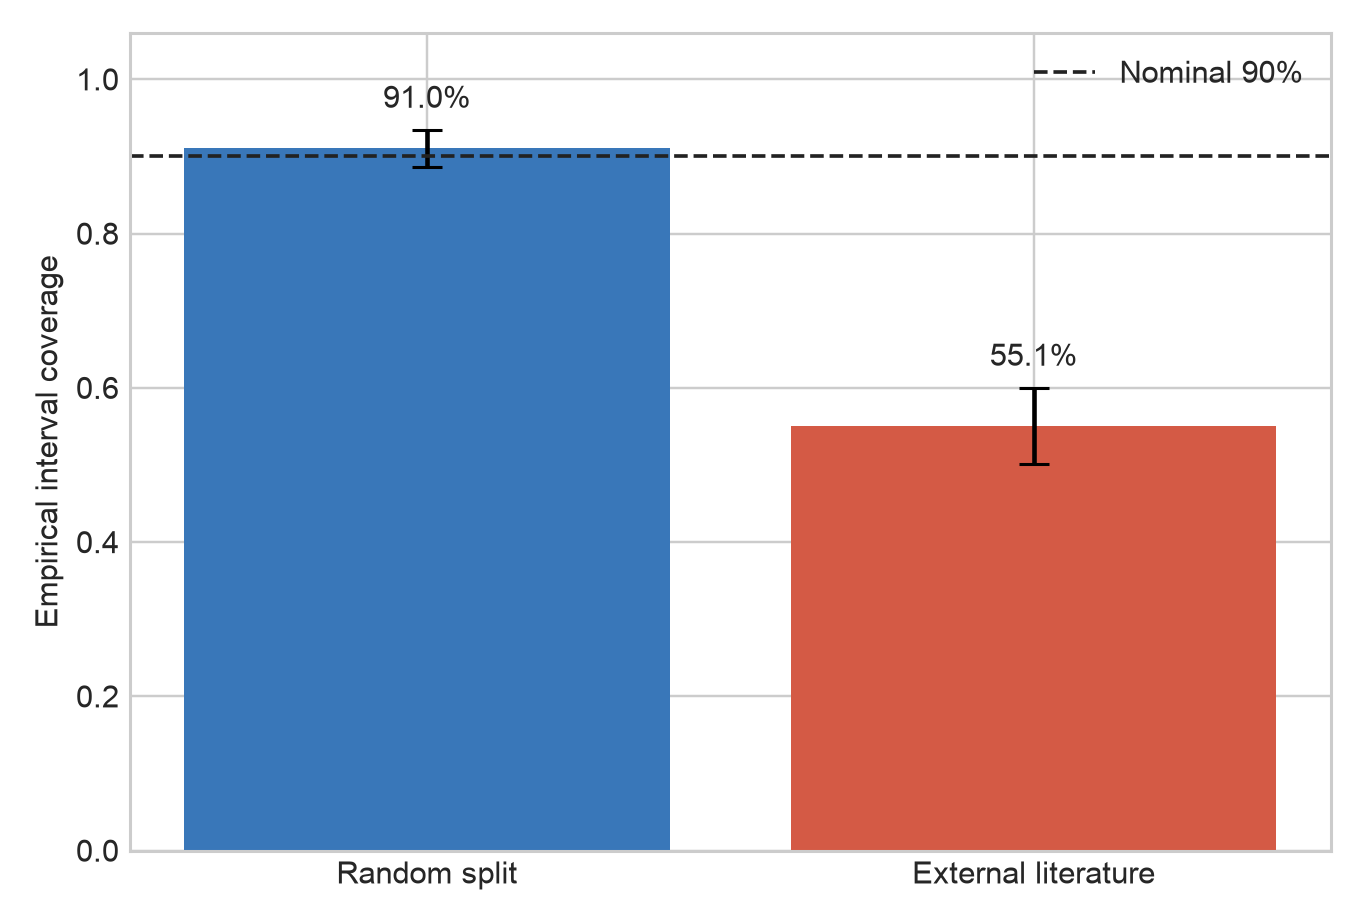
\includegraphics[width=0.8\linewidth]{figure_cqr_coverage_shift}
\caption{内部随机测试行与外部文献集上名义 90\% CQR 覆盖率的对比(15 次运行)。}
\label{fig:cqr}
\end{figure}

\subsection{R4:无标签适用域剪枝(试点规则与规范规则)}
\label{sec:r4}

\paragraph{试点规则(Pilot rule)} 仅使用 868 个训练输入,我们将八个特征标准化,计算留一法(leave-one-out)5 近邻(5-NN)距离,并取其第 95 百分位数(0.9572)作为阈值。在 64 个外部候选中,26 个被保留、38 个被剪除(剪枝率 59.375\%,缩减 $2.46\times$)。距离与绝对误差相关(Spearman $\rho=0.718$,$p=2.46\times10^{-11}$,按行朴素计算;图~\ref{fig:distance})。保留的候选 MAE 为 4.87 µm,被剪除者为 17.26 µm。在 10 µm 容差下,全部 64 个外部候选中有 38 个成功(59.4\%);在 26 个保留候选中有 24 个成功(92.3\%);因此成功候选的召回率为 24/38 = 63.2\%。在 15 和 20 µm 下,保留精度为 1.0,召回率分别为 0.591 和 0.553。分母不同,不得混淆:59.4\% 是相对于全部外部候选,92.3\% 是相对于保留候选。保留完全按来源分块——Galogahi 0/24、Roumpea 0/14、Lashkaripour 20/20、Mazutis 6/6——因此试点规则剔除的是整个文献来源,而非个别候选(图~\ref{fig:pruning})。

\paragraph{规范规则(Canonical rule)} 在冻结的扩展套件(第~\ref{sec:expanded}~节)中,阈值是在依赖分组的留出校准分区(104 个单乳液行)上校准的,而不是基于留一法训练得分,5-NN 阈值变为 1.5647。该规则随后保留 64 个候选中的 32 个(Galogahi 6/24、Lashkaripour 20/20、Mazutis 6/6、Roumpea 0/14)。在 10 µm 容差下,其精度为 93.8\%(30/32),召回率为 78.9\%(30/38);在 10\% 相对误差下,其精度为 62.5\%,召回率为 71.4\%,而全池成功率为 43.8\%(28/64)。表~\ref{tab:pruning} 并列给出两条规则。H3 的精度部分得到支持,但第~\ref{sec:r7}~节中考虑依赖关系的对照限定了其机制。

\begin{table}[t]
\centering\small
\caption{对 64 个外部候选的无标签 5-NN 剪枝:试点规则(留一法训练阈值)与规范规则(依赖分组校准阈值)。精度针对保留候选计算;召回率针对完整候选池中全部成功候选计算。}
\label{tab:pruning}
\resizebox{\linewidth}{!}{%
\begin{tabular}{lrr}
\toprule
 & 试点(LOO q95) & 规范(分组 q95) \\
\midrule
阈值(标准化距离) & 0.9572 & 1.5647 \\
保留 / 剪除 & 26 / 38 & 32 / 32 \\
分来源保留(G/L/M/R) & 0/24, 20/20, 6/6, 0/14 & 6/24, 20/20, 6/6, 0/14 \\
全池成功率,10 µm & 59.4\% (38/64) & 59.4\% (38/64) \\
保留精度,10 µm & 92.3\% (24/26) & 93.8\% (30/32) \\
成功候选召回率,10 µm & 63.2\% (24/38) & 78.9\% (30/38) \\
保留精度 / 召回率,10\% 相对误差 & — & 62.5\% / 71.4\% \\
\bottomrule
\end{tabular}}
\end{table}

\begin{figure}[t]
\centering
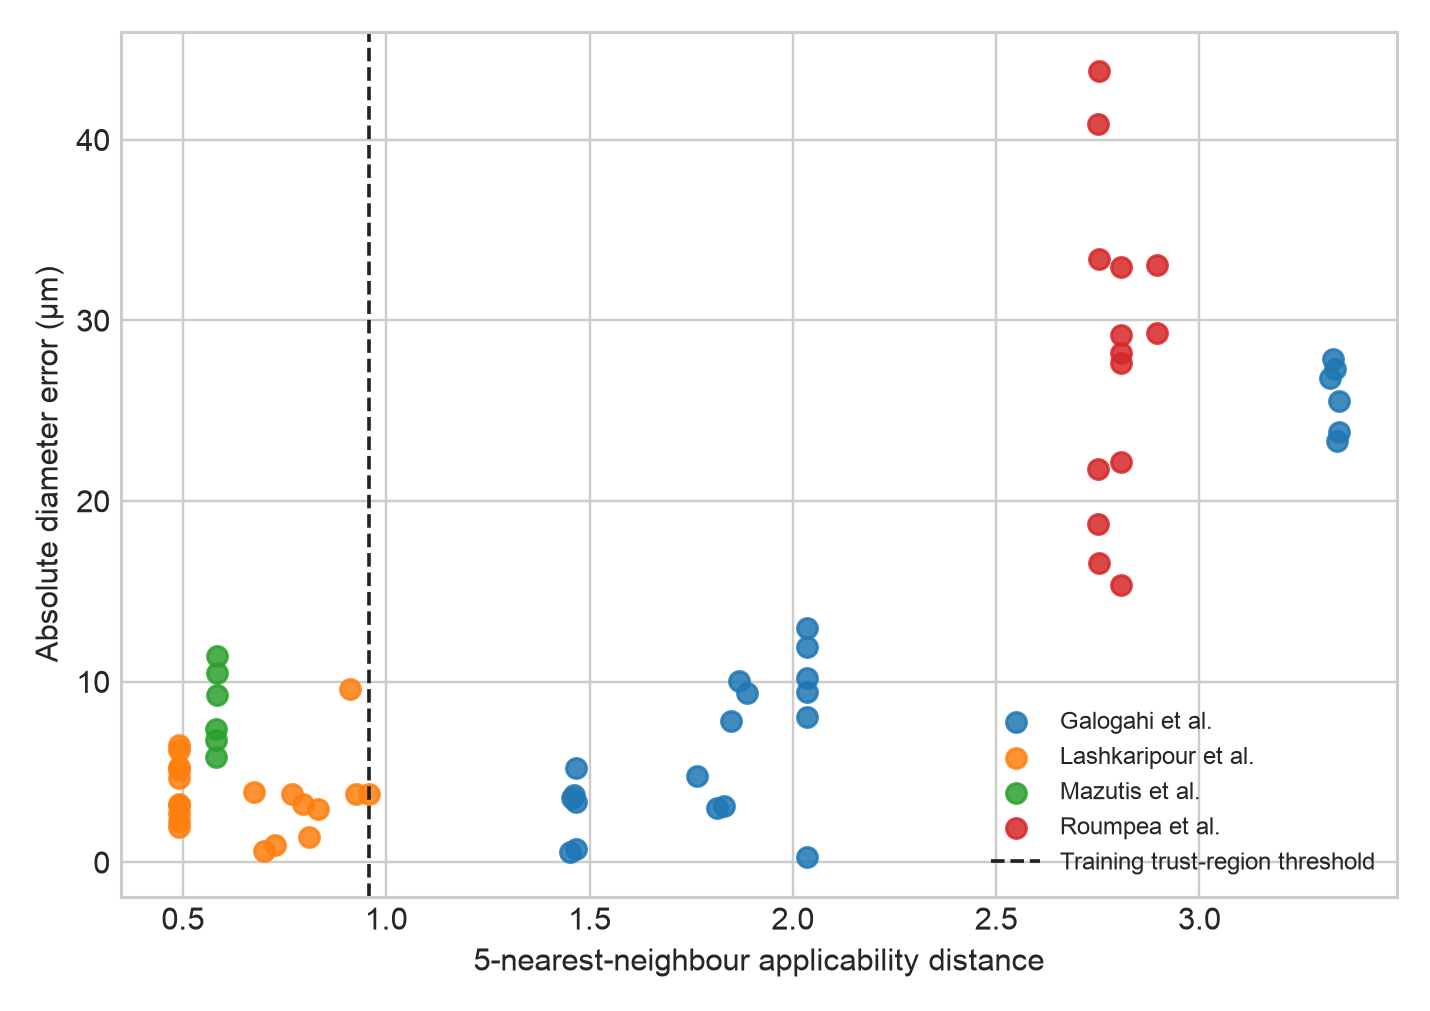
\includegraphics[width=0.75\linewidth]{figure_distance_vs_error}
\caption{试点规则:到训练输入的标准化 5-NN 距离与外部绝对误差的关系,并标出第 95 百分位阈值。}
\label{fig:distance}
\end{figure}

\begin{figure}[t]
\centering
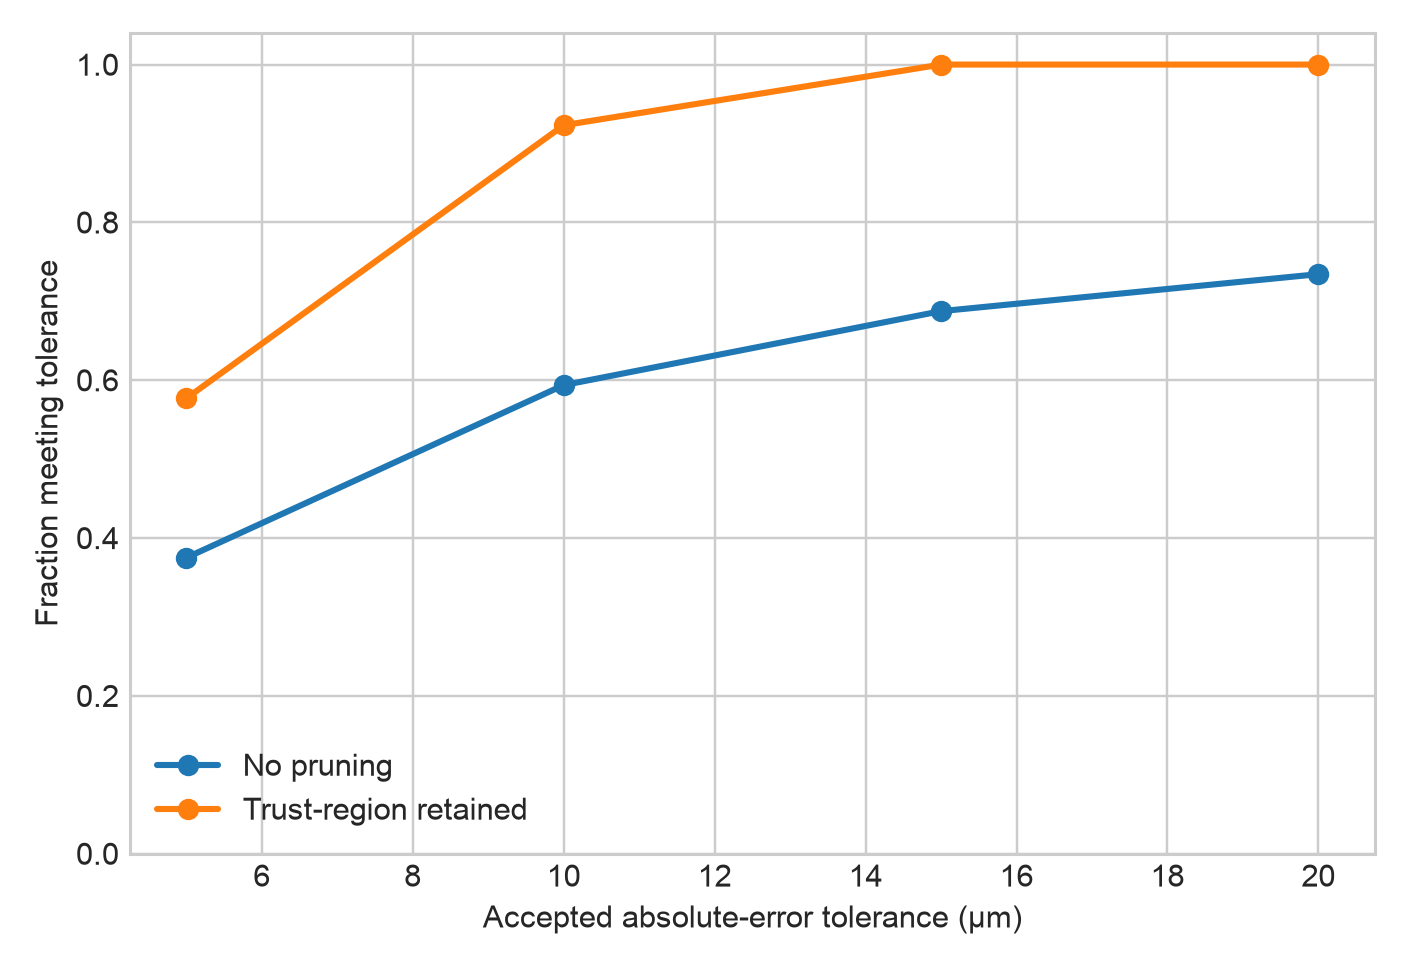
\includegraphics[width=0.75\linewidth]{figure_pruning_precision}
\caption{试点规则:剪枝前后处于容差内的候选比例。精度上升而召回率下降;二者必须结合解读。}
\label{fig:pruning}
\end{figure}

\subsection{R5:密封 TX100 验证——负结果}
\label{sec:r5}

表~\ref{tab:v1} 列出每一项锁定的终点。冻结的点模型在 87 个 TX100 行上的盲测 MAPE 为 19.8436\%,未满足两项预先声明的判据(复现 $<11.4\%$:不成立;强复制 $\le 6\%$:不成立),MAE 为 0.022615 mm,RMSE 为 0.028681 mm,$R^2=-0.2436$(约 $-0.24$)。90\% 分割共形区间覆盖了 0.4483 的行(平均宽度 0.03281 mm)。揭盲后的描述性分析发现 85.06\% 的行被高估,带符号相对偏差为 0.1895;在这 87 行的条件下,行自助法(row bootstrap)将 MAPE 置于 $[16.4\%, 23.5\%]$,覆盖率的 Wilson 区间为 $[0.348, 0.553]$。严格的 min–max 筛选接受了全部 87 行(候选缩减 0.0):失败并非边际范围越界,而是条件偏移(conditional shift)——四个记录的预测变量与训练支撑重叠,而它们与直径的关系随未见过的表面活性剂而改变(图~\ref{fig:v1diag})。

在锁定的适用域规则中,只有孤立森林(Isolation Forest)满足全部四项预先声明的收益条件(候选缩减 0.1034,保留相对风险 0.1861,而全池为 0.1984,等预算单侧 $p=0.0266$,在 0.05 水平下成立);5-NN($p=0.111$)和马氏距离(Mahalanobis,$p=0.675$)则不满足。然而,在对四项锁定检验作 BH(Benjamini–Hochberg)校正之后,孤立森林的结果不再显著(校正后 $p=0.106$),因此我们仅将其报告为提示性结果(图~\ref{fig:v1risk})。六种目标搜索策略回答了同样的 13 个固定目标中的 8 个(覆盖率 0.615),在全部查询上 success@1 为 0.2308,success@3/@5 为 0.4615/0.6154,oracle 可达召回率在 1/3/5 处为 0.25/0.50/0.667;筛选并未改变排名第一的候选,仅马氏距离在一次查询上例外。独立重算与恢复所得结果在每个指标上的一致性均在 $10^{-12}$ 以内,且所有冻结的来源哈希在揭盲后分析前后均未改变。

\paragraph{回顾性开发参照(事后)} 预先声明的阈值以源论文的分布内数值为锚(第~\ref{sec:v1protocol}~节)。按后来用于 D3 的开发侧判据,锁定的 V1 模型在五个开发组上的留一化学体系(leave-one-chemistry-out)MAPE 为:6.54\%(CMC 0,$n=63$)、5.01\%(2 mM,30)、15.76\%(4.33 mM,15)、5.46\%(11 mM,178)和 6.46\%(20 mM,93):宏平均 7.85\%,汇总 6.26\%,另有 2 行 CMC 未列出的行仅保留在训练侧。$1.25\times$ 复现阈值本应为 9.81\%;密封的 19.8436\% 是宏参照的 2.53 倍,同样不满足该判据。因此,无论按预先登记的判据还是回顾性判据,结果均为负,且 TX100 误差超过每一个开发折,最接近的是 15 行的 4.33 mM 组,为 15.76\%。

\begin{table}[t]
\centering\small
\caption{密封 TX100 组($n=87$)上锁定的 V1 终点。}
\label{tab:v1}
\begin{tabular}{lr}
\toprule
终点 & 值 \\
\midrule
MAPE & 19.8436\% \\
复现判据($<11.4\%$) & 未满足 \\
强复制判据($\le 6.0\%$) & 未满足 \\
MAE / RMSE & 0.022615 / 0.028681 mm \\
$R^2$ & $-0.2436$ \\
名义 90\% 覆盖率(平均宽度) & 0.4483 (0.03281 mm) \\
被高估的行 & 85.06\% \\
带符号相对偏差 & 0.1895 \\
严格 min–max 候选缩减 & 0.0 \\
孤立森林 q95:缩减 / $p$ / BH $p$ & 0.1034 / 0.0266 / 0.106 \\
已回答的目标查询 & 13 个中的 8 个 \\
Success@1 / @3 / @5(全部查询) & 0.2308 / 0.4615 / 0.6154 \\
\bottomrule
\end{tabular}
\end{table}

\begin{figure}[t]
\centering
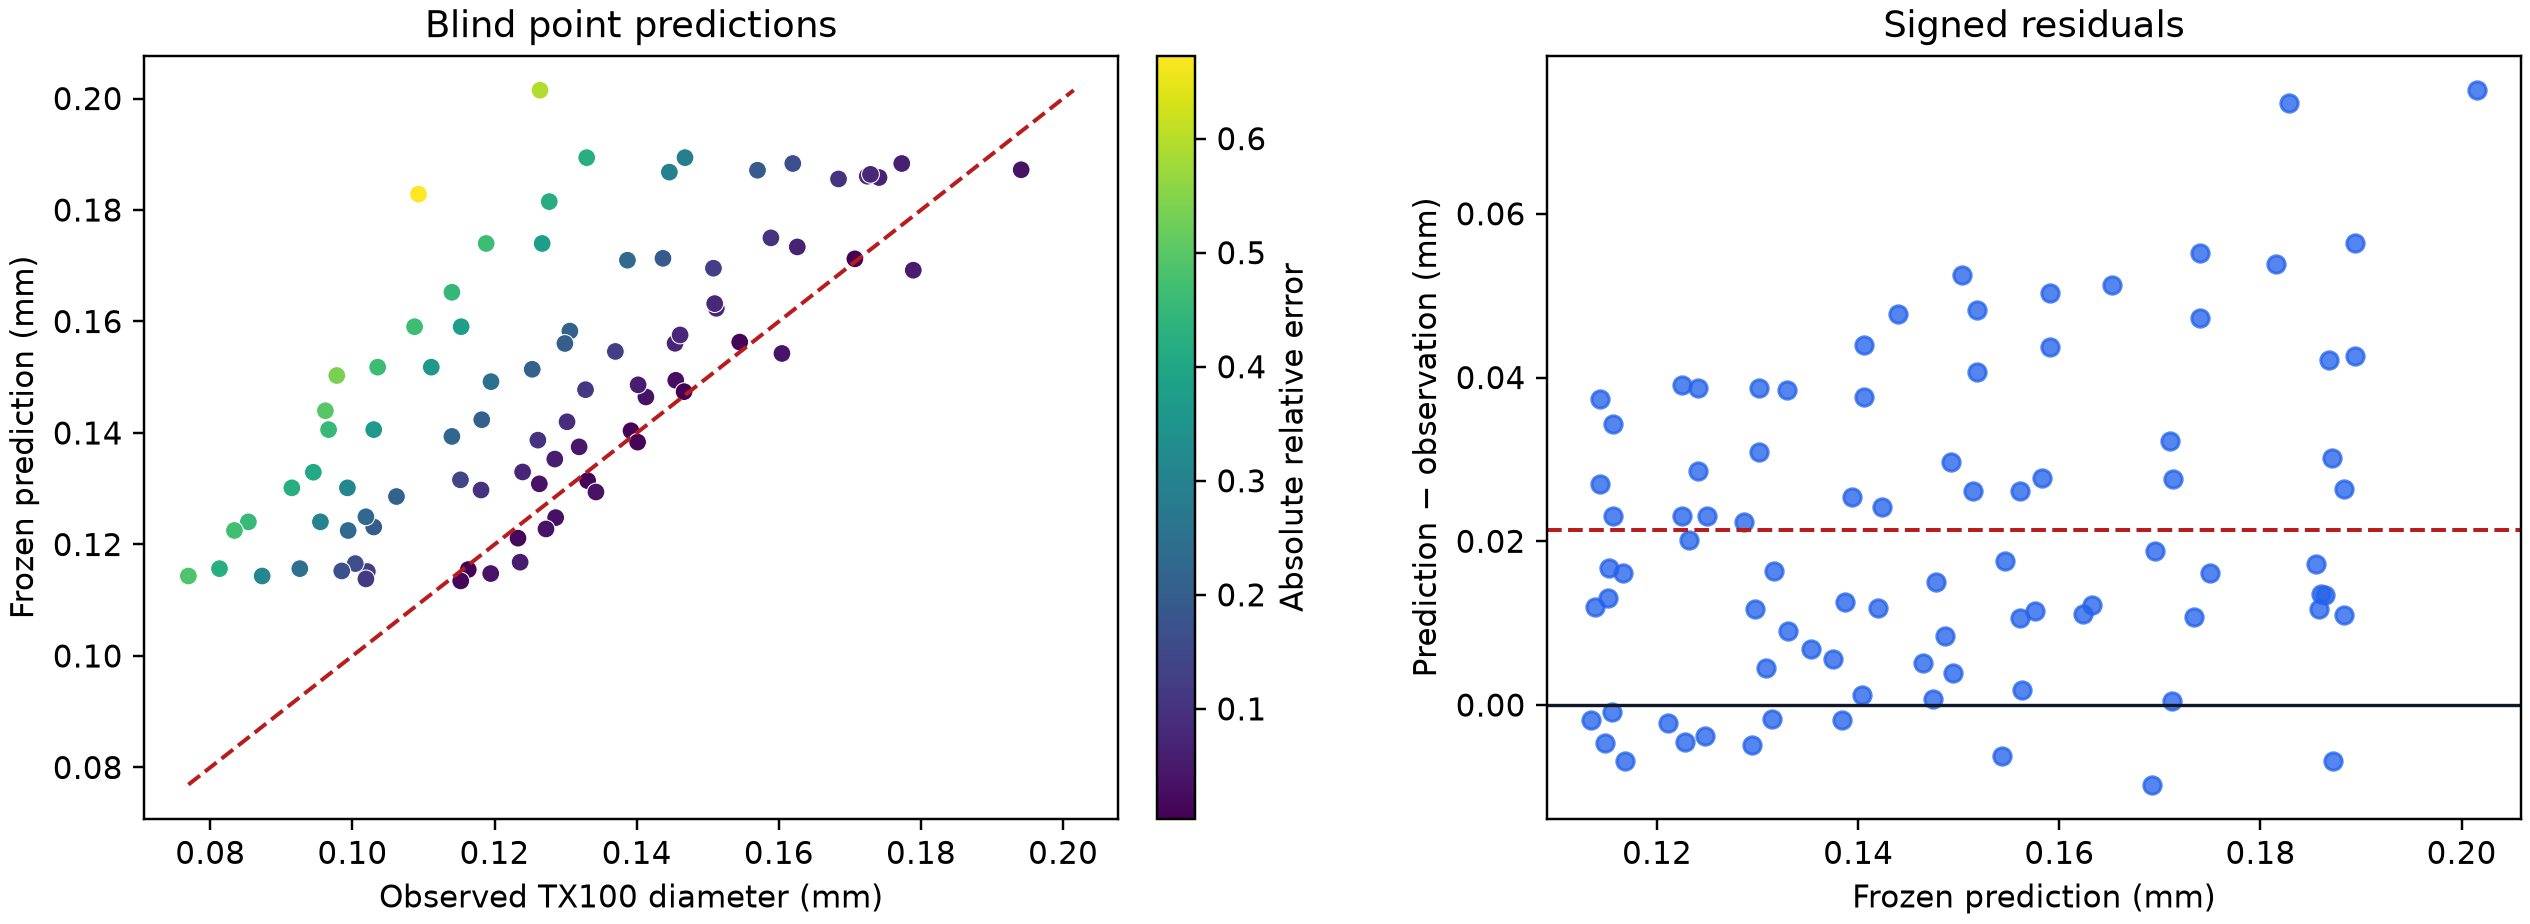
\includegraphics[width=\linewidth]{v1_figure_1_blind_prediction_diagnostics}
\caption{负结果。左:冻结的 V1 预测与观测的 TX100 直径(87 行)的对比,按绝对相对误差着色。右:带符号残差与预测值的关系;虚线为平均偏差(0.0213 mm)。}
\label{fig:v1diag}
\end{figure}

\begin{figure}[t]
\centering
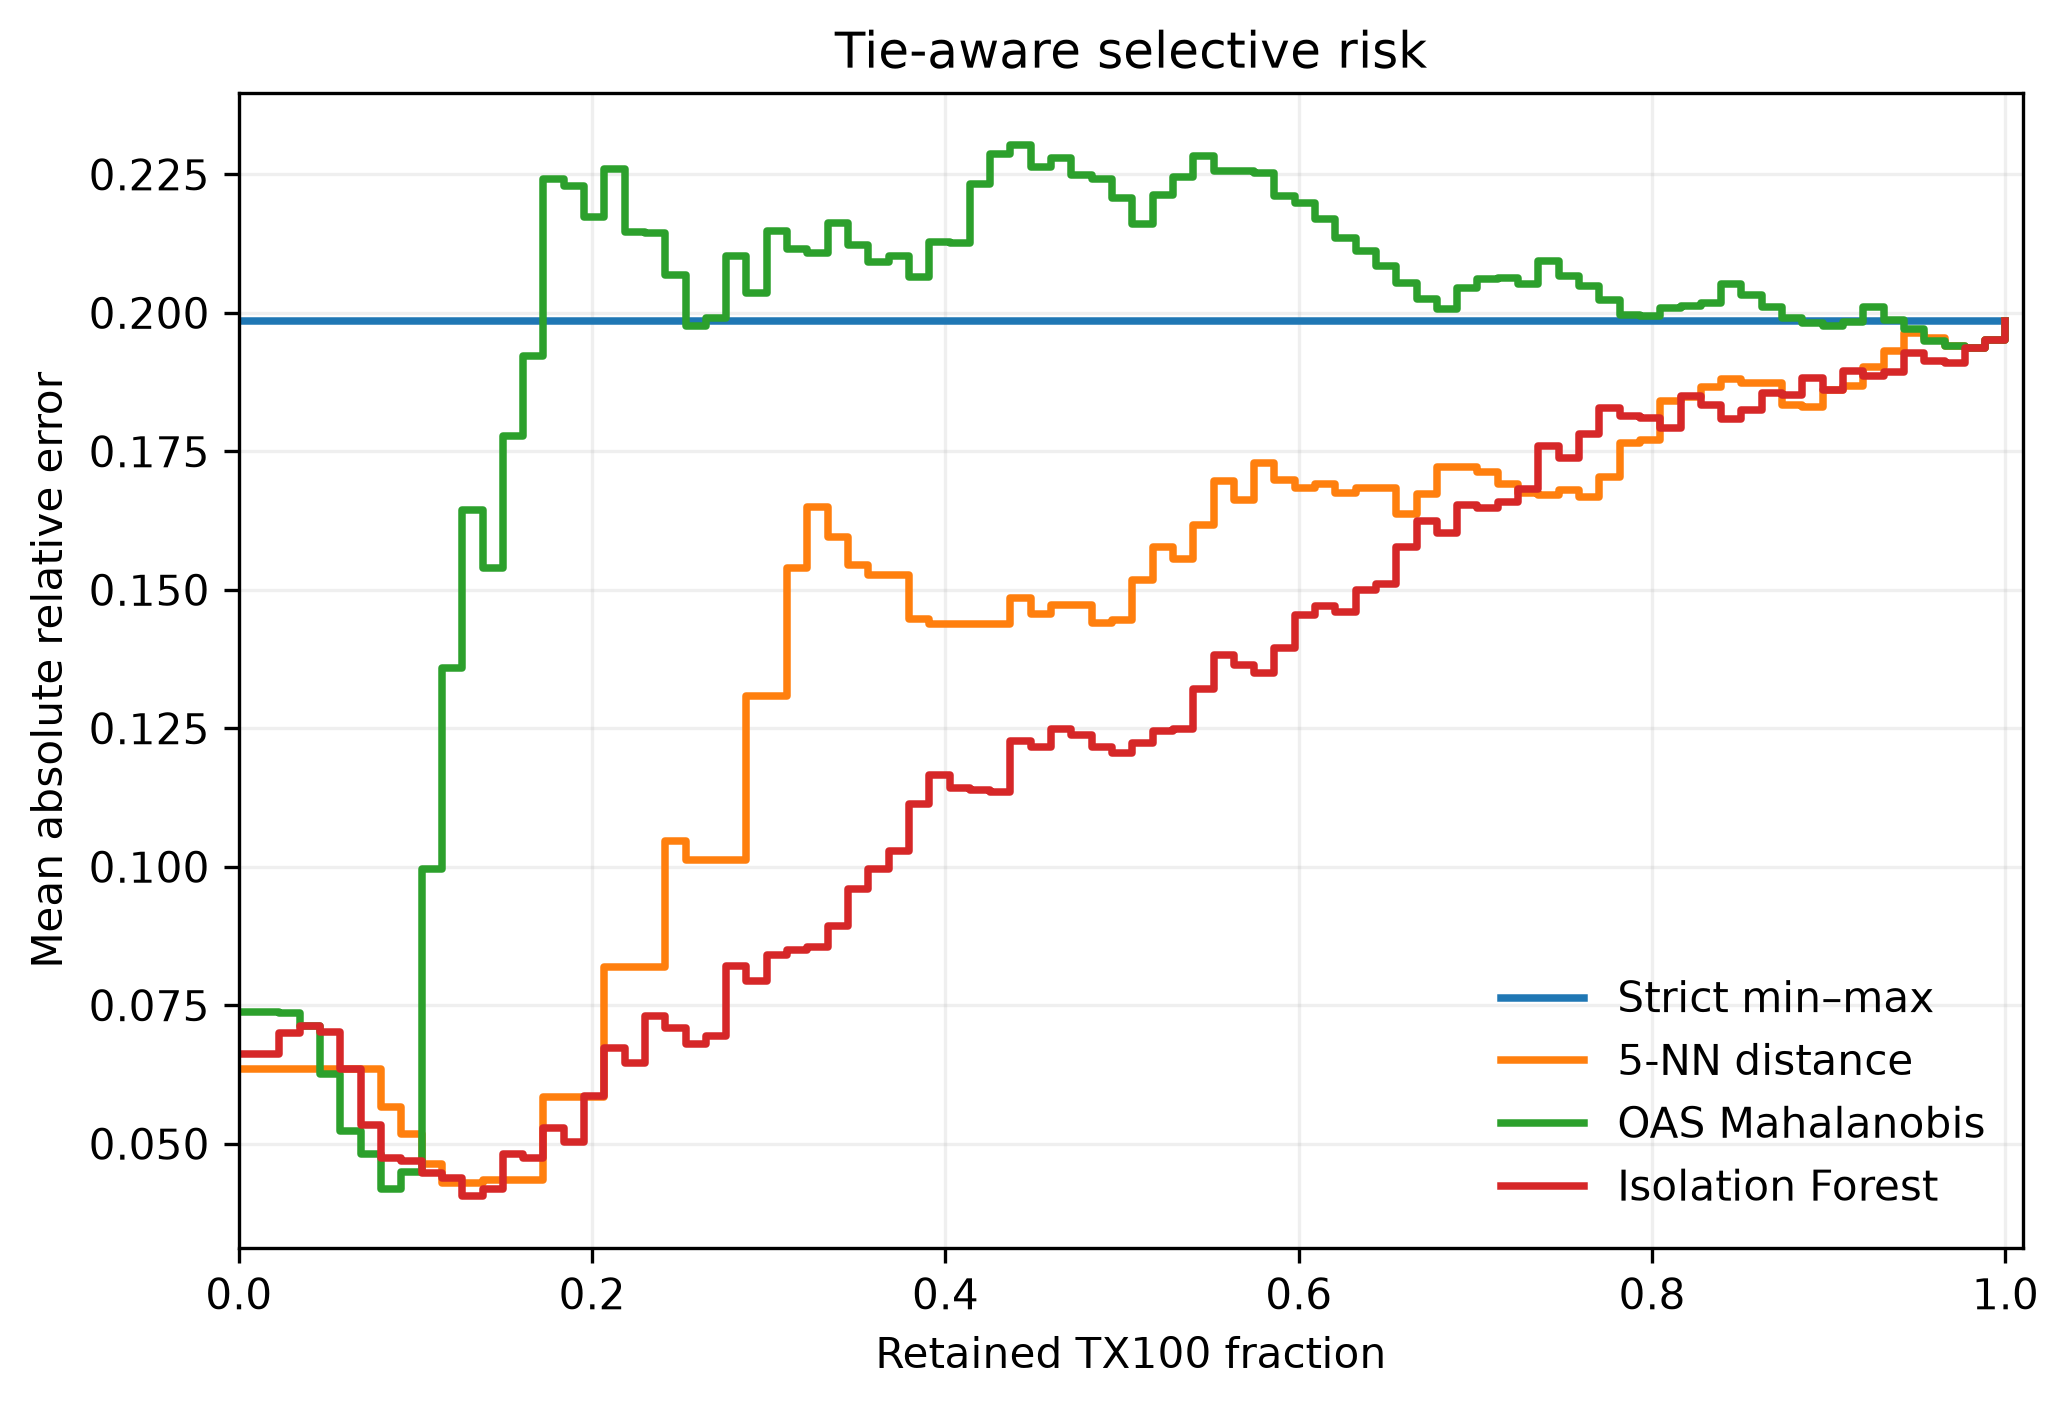
\includegraphics[width=0.8\linewidth]{v1_figure_2_blind_risk_coverage}
\caption{负结果,适用域视角。四种锁定筛选在 TX100 行上的并列感知(tie-aware)选择性风险。没有任何筛选能在不付出大幅保留损失的情况下把保留风险降到全池风险以下;唯一预先声明的收益(孤立森林)在 BH 校正后不成立。}
\label{fig:v1risk}
\end{figure}

\subsection{R6:V2 回顾性结果——负/混合裁决}
\label{sec:r6}

两次完整的规范运行在不同目录中产生了逐字节相同的产物哈希清单(artifact-hash manifests)。表~\ref{tab:v2} 给出模型矩阵。对照冻结的决策规则,条件 1 未通过:V2-P 化学体系宏 MAPE 为 12.0496\%,而 B1 为 10.2680\%。条件 2 未通过:V2-P 仅在 6 个留出组中的 2 个上优于 B1(CMC 3.5 mM,即揭盲后的 TX100 组,$-8.138$ pp;CMC 4.33 mM,$-1.011$ pp;要求四个组;图~\ref{fig:v2paired})。条件 3–6 成立:V2-P 的最差组为 14.847\%,B1 为 19.960\%;V2-H、V2-M 和 V2-P 的点预测与区间物理无效率均为零,而 B1 为 3.22\%,无约束的 B3 为 13.73\%;回顾性检索同时报告覆盖率、召回率和精度;没有任何外层结果被用于选择。锁定的决策文件记录了 \texttt{beneficial\_claim\_allowed = false}:V2-P 未达到预先登记的整体优越性判据,因此裁决为混合。硬结构边界并未相对于 B1 降低化学体系宏平均误差,但在这些回顾性分析中消除了全部物理无效的点预测,并缩小了最差组误差。

原生输入 XGBoost 消融 B2 的化学体系宏 MAPE 为 9.13\%,B1 为 10.27\%;这是在单一协议下作为消融报告的,不归因于 V2。V2 的有界 LOCO 折外不确定性启发式在留出组上的平均覆盖率为 0.744(V2-P),作为无名义保证的迁移压力测试。回顾性约束检索在几乎所有查询上都弃权:在 10\% 相对容差下,B3 和 V2-H 在 78 个查询中回答了 1 个,其余每个模型均未回答;在 0.01 mm 绝对容差下,没有任何模型回答任何查询。我们将其作为空检索终点(null search endpoint)报告,而不是省略。

\begin{table}[t]
\centering\small
\caption{嵌套留一化学体系评估下冻结的 V2 模型矩阵(466 行,六个组,五个种子;TX100 为揭盲后回顾性)。}
\label{tab:v2}
\resizebox{\linewidth}{!}{%
\begin{tabular}{lrrrrr}
\toprule
模型 & 宏 MAPE & 最差组 & 行 MAPE & 点预测无效 & 区间无效 \\
\midrule
B0 锚点方程 & 18.38\% & 28.31\% & 13.99\% & 1.29\% & — \\
B1 四输入 XGBoost & 10.27\% & 19.96\% & 9.12\% & 3.22\% & — \\
B2 原生输入 XGBoost & 9.13\% & 16.94\% & 8.86\% & 2.58\% & — \\
B3 原生+物理 MLP(无界) & 16.64\% & 32.50\% & 14.45\% & 13.73\% & 0 \\
V2-H 有界 MLP & 10.59\% & 14.63\% & 10.72\% & 0 & 0 \\
V2-M V2-P + 单调惩罚 & 12.05\% & 14.84\% & 11.30\% & 0 & 0 \\
V2-P 有界残差 + 锚点(主要) & 12.05\% & 14.85\% & 11.30\% & 0 & 0 \\
\bottomrule
\end{tabular}}
\end{table}

\begin{figure}[t]
\centering
\begin{tikzpicture}
\begin{axis}[
  width=0.8\linewidth, height=6cm, ybar, bar width=14pt,
  ylabel={V2-P 减 B1 的 MAPE(pp)},
  xlabel={留出化学体系组(CMC,mM)},
  xtick=data, xticklabels={0, 2, {3.5 (\tox{})}, 4.33, 11, 20},
  x tick label style={font=\small},
  ymajorgrids, grid style={dashed,gray!30},
  nodes near coords, nodes near coords style={font=\scriptsize,/pgf/number format/fixed,/pgf/number format/precision=2},
  enlarge x limits=0.12,
]
\addplot+[fill=gray!60, draw=black] table[col sep=comma, x expr=\coordindex,
  y=V2_P_minus_B1_mape_percentage_points]{data/paired_group_differences_v2p_vs_b1.csv};
\draw[black] (axis cs:-0.5,0) -- (axis cs:5.5,0);
\end{axis}
\end{tikzpicture}
\caption{负/混合结果。六个化学体系组上留出组 MAPE 的配对差,V2-P 减 B1(负值有利于 V2-P)。TX100 组是揭盲后的回顾性分析,而非盲测。V2-P 仅赢得两个组,未满足锁定条件 2。}
\label{fig:v2paired}
\end{figure}

\subsection{R7:DAFD 上的扩展偏移诊断与负对照}
\label{sec:r7}

\paragraph{分组划分(Grouped splits)} 对于焦点 XGBoost 模型,直径 MAPE 的均值在行随机划分上为 5.27\%,在精确输入分组划分上为 5.74\%,在几何分组划分上为 11.69\%(中位数 11.07\%,30 次划分的范围为 6.39–23.58\%),在几何加流体分组划分上为 10.18\%(图~\ref{fig:splits})。行随机划分存在泄漏:平均有 79\% 的双乳液配对跨越训练/测试边界,99.5\% 的测试几何出现在训练中。随机森林与直方图梯度提升呈现相同模式(5.81/6.32/10.67/9.39\% 和 5.01/5.41/11.33/10.12\%)。打乱标签的对照给出外部 MAPE 33.4\%(30 个种子的范围为 23.0–46.8\%),证实模型学到了信号。等权来源宏平均(source-macro)外部 MAPE,XGBoost 为 13.21\%,而按行微平均为 11.26\%。

\paragraph{区间迁移(Interval transfer)} 在扩展套件的校准协议下,采用行级随机校准时,名义 90\% CQR 覆盖率由内部的 0.900 降至外部的 0.521(平均宽度由 28.3 增至 34.1 µm);分割共形与归一化分割共形表现类似(0.908 $\to$ 0.469;0.912 $\to$ 0.524)。采用几何分组校准时,外部 CQR 覆盖率为 0.848,平均宽度 89.8 µm,分割共形为 0.890(66.7 µm),归一化分割共形为 0.936(104.2 µm);CQR 的等权来源宏平均外部覆盖率为 0.750,同时依赖组覆盖率为 0.714。因此,分组校准以大约三倍的区间宽度换取覆盖率,并且由于校准组数量少而存在 0.95 的有限样本上限。

\paragraph{适用域得分与对照(Applicability scores against controls)} 在连续相对风险曲线上,全池平均绝对相对误差为 0.1126,AURC(风险—覆盖曲线下面积)值为 0.1053(5-NN)、0.0951(马氏距离)、0.1082(孤立森林)和 0.109(随机得分)。仅用水力直径的对照达到 0.0734,单类 SVM(one-class SVM)为 0.0882;折外残差风险模型(0.1431)和自助分歧(bootstrap disagreement,0.1273)比随机更差。由于在连续相对风险上没有任何适用域得分优于仅用尺寸的对照,在我们预先登记的判据下,它们中没有任何一个能支持候选级收益声明(图~\ref{fig:riskcov})。相较等预算随机保留,q95 处的二值 5-NN 规则确实降低了保留相对风险(0.0961 对 0.1126)(全局 $p=0.020$,BH 0.036;按来源分层 $p=0.0013$,BH 0.0039;来源内物理簇置换 $p=0.0030$,BH 0.0076),但在保持“保留哪些上下文”不变的来源内上下文置换(within-source-context permutation)下,该效应消失($p=1.0$):收益可由规则保留了哪些来源上下文来解释(图~\ref{fig:retention})。5-NN 距离与相对误差的总体 Spearman 相关为 0.222($p=0.078$,按行朴素计算),且在各来源内符号相反(Galogahi 0.79,Lashkaripour $-0.27$,Roumpea $-0.49$),而仅水力直径与相对误差的相关为 0.69。保留减全池相对风险的先来源后簇分层自助(source-then-cluster hierarchical bootstrap)区间,对 5-NN($-0.016$,95\% 区间 $[-0.088, 0.027]$)和马氏距离($-0.021$,$[-0.056, 0.021]$)均包含零。

\paragraph{回顾性目标搜索重放(Retrospective target-search replay)} 在按来源池划分的 84 个上下文–目标查询上(其中 30 个在 10\% 相对容差下 oracle 可达),未筛选的点排序回答了 26.2\% 的查询,success@1 精度为 0.50,成功目标召回率为 0.367(success@3:0.636/0.467)。5-NN q95 筛选将已回答精度提高到 0.60,但仅回答 6.0\% 的查询,召回率为 0.10;马氏距离与严格 min–max 筛选回答 14.3\%,精度 0.667,召回率 0.267;共形目标包含(conformal target inclusion)回答 25.0\%,精度 0.524,召回率 0.367;同分位数下的随机得分筛选回答 26.2\%,精度 0.455,召回率 0.333。筛选以查询覆盖率和召回率换取精度,且从未在三项终点上同时支配未筛选或随机策略。

\begin{figure}[t]
\centering
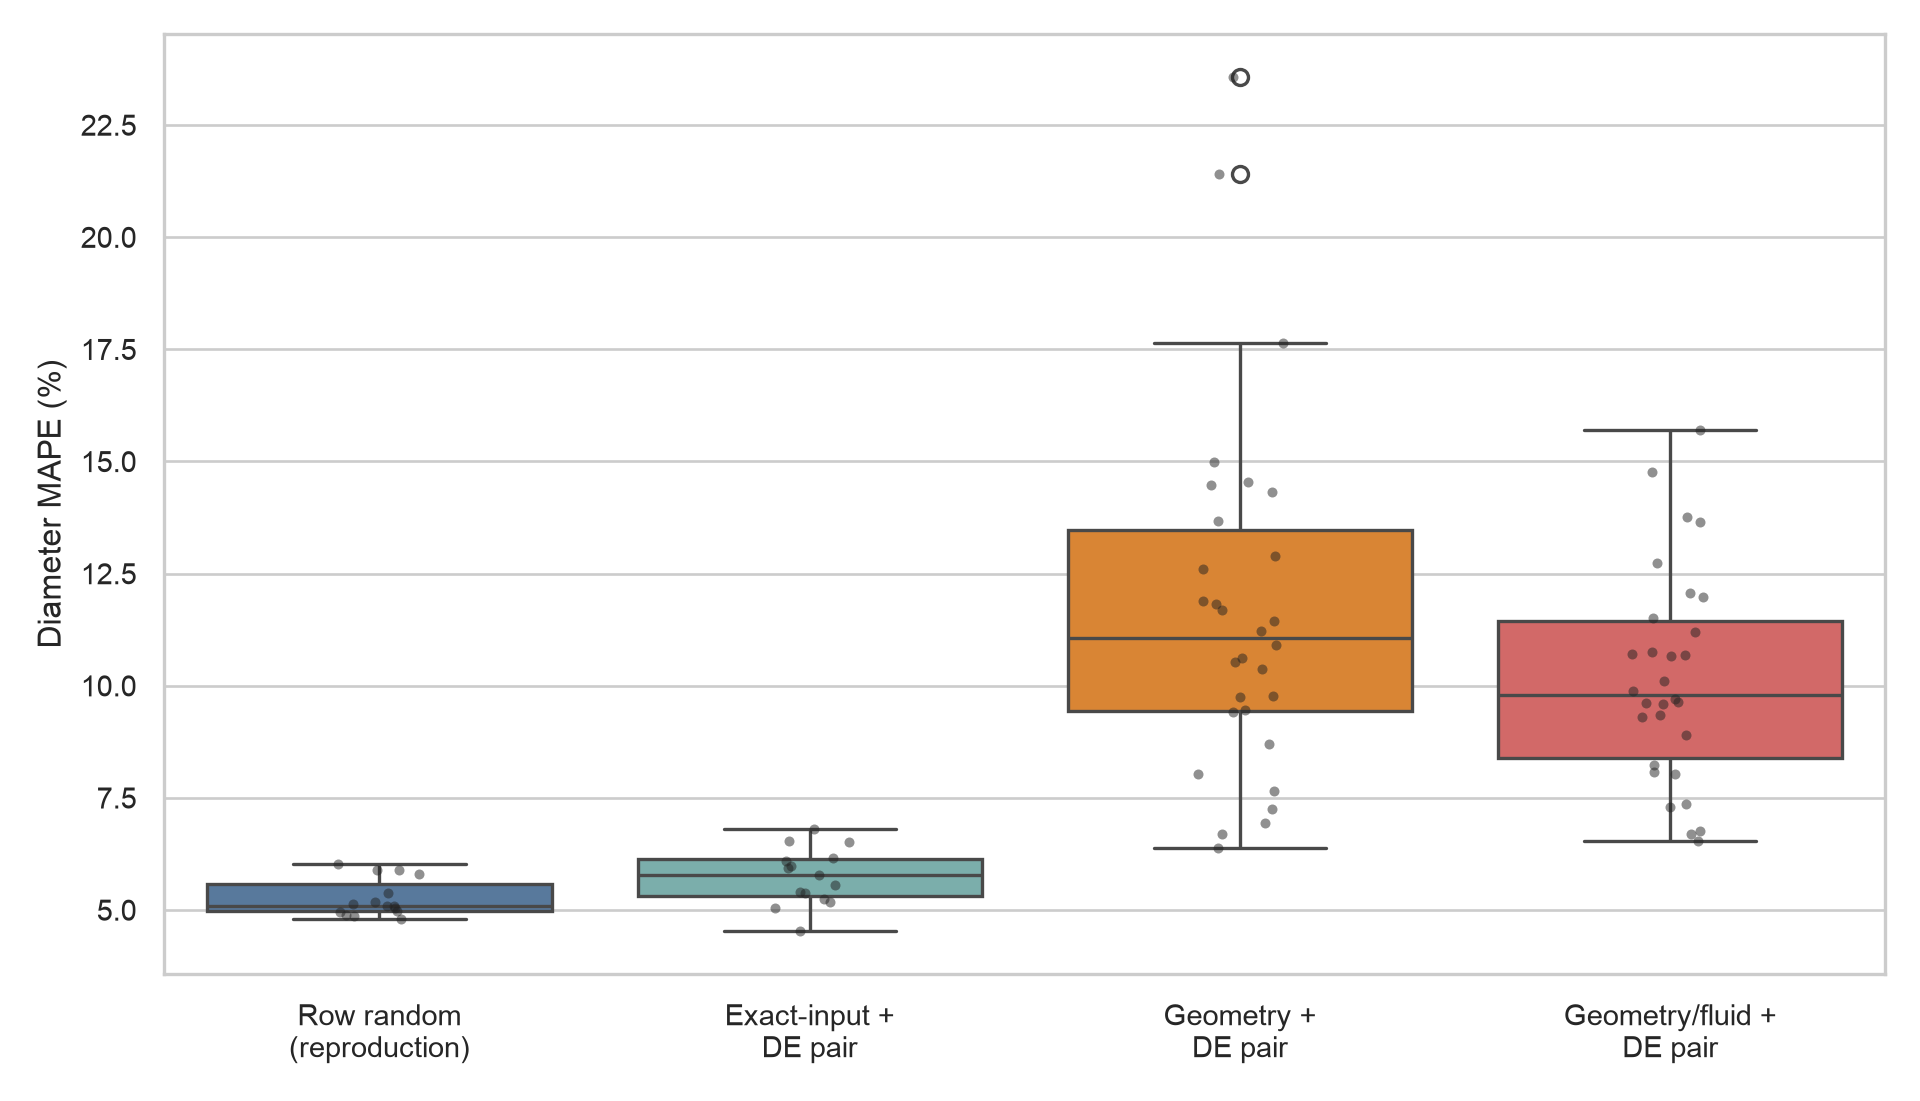
\includegraphics[width=0.85\linewidth]{expanded_figure_1_split_generalization}
\caption{焦点 XGBoost 在 868 行表上四种划分协议下的直径 MAPE。分组协议避免双乳液配对与器件几何跨越拟合/测试边界。}
\label{fig:splits}
\end{figure}

\begin{figure}[t]
\centering
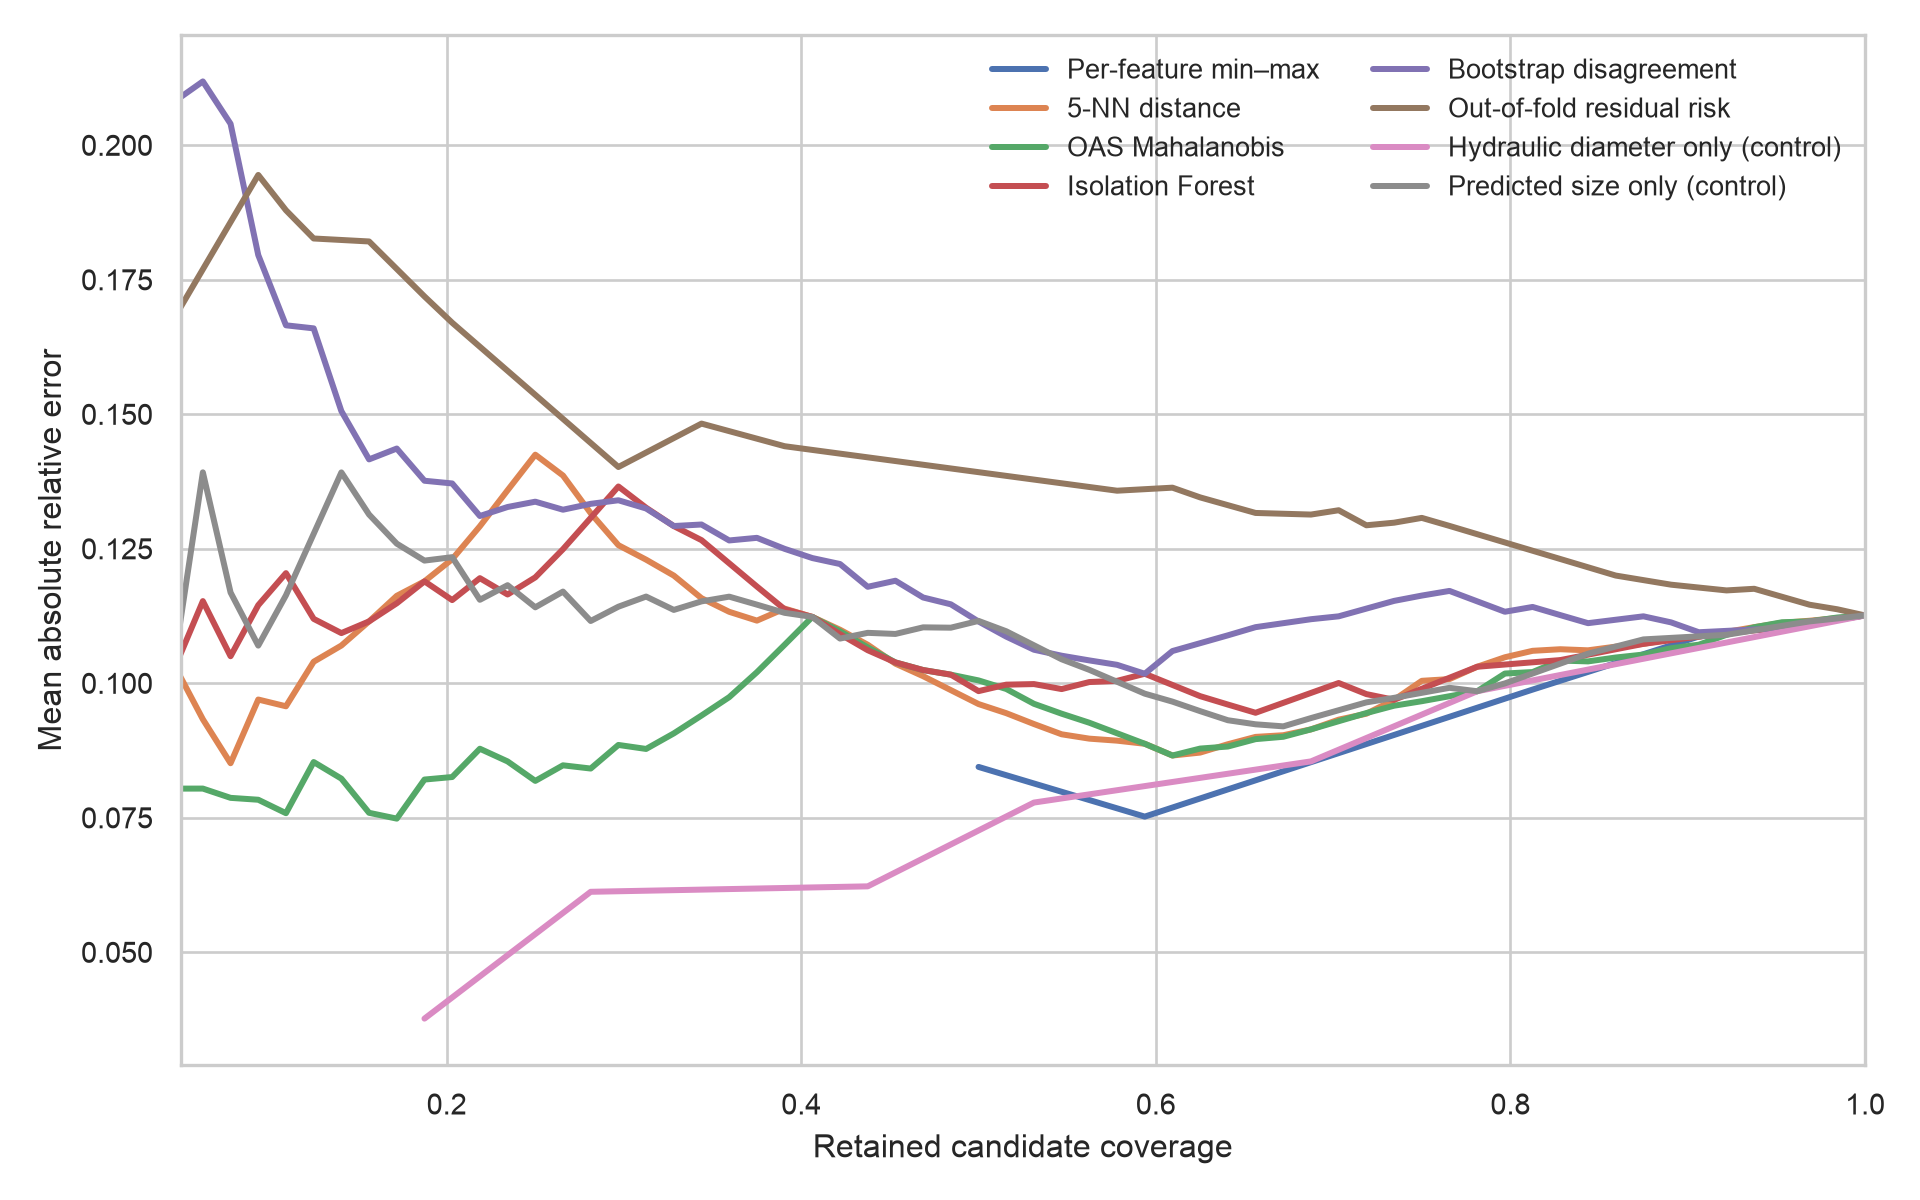
\includegraphics[width=0.85\linewidth]{expanded_figure_3_relative_risk_coverage}
\caption{64 个外部行上适用域得分与对照的相对风险—保留覆盖率曲线。仅用水力直径的对照具有最低 AURC;没有任何无标签适用域得分优于它。}
\label{fig:riskcov}
\end{figure}

\begin{figure}[t]
\centering
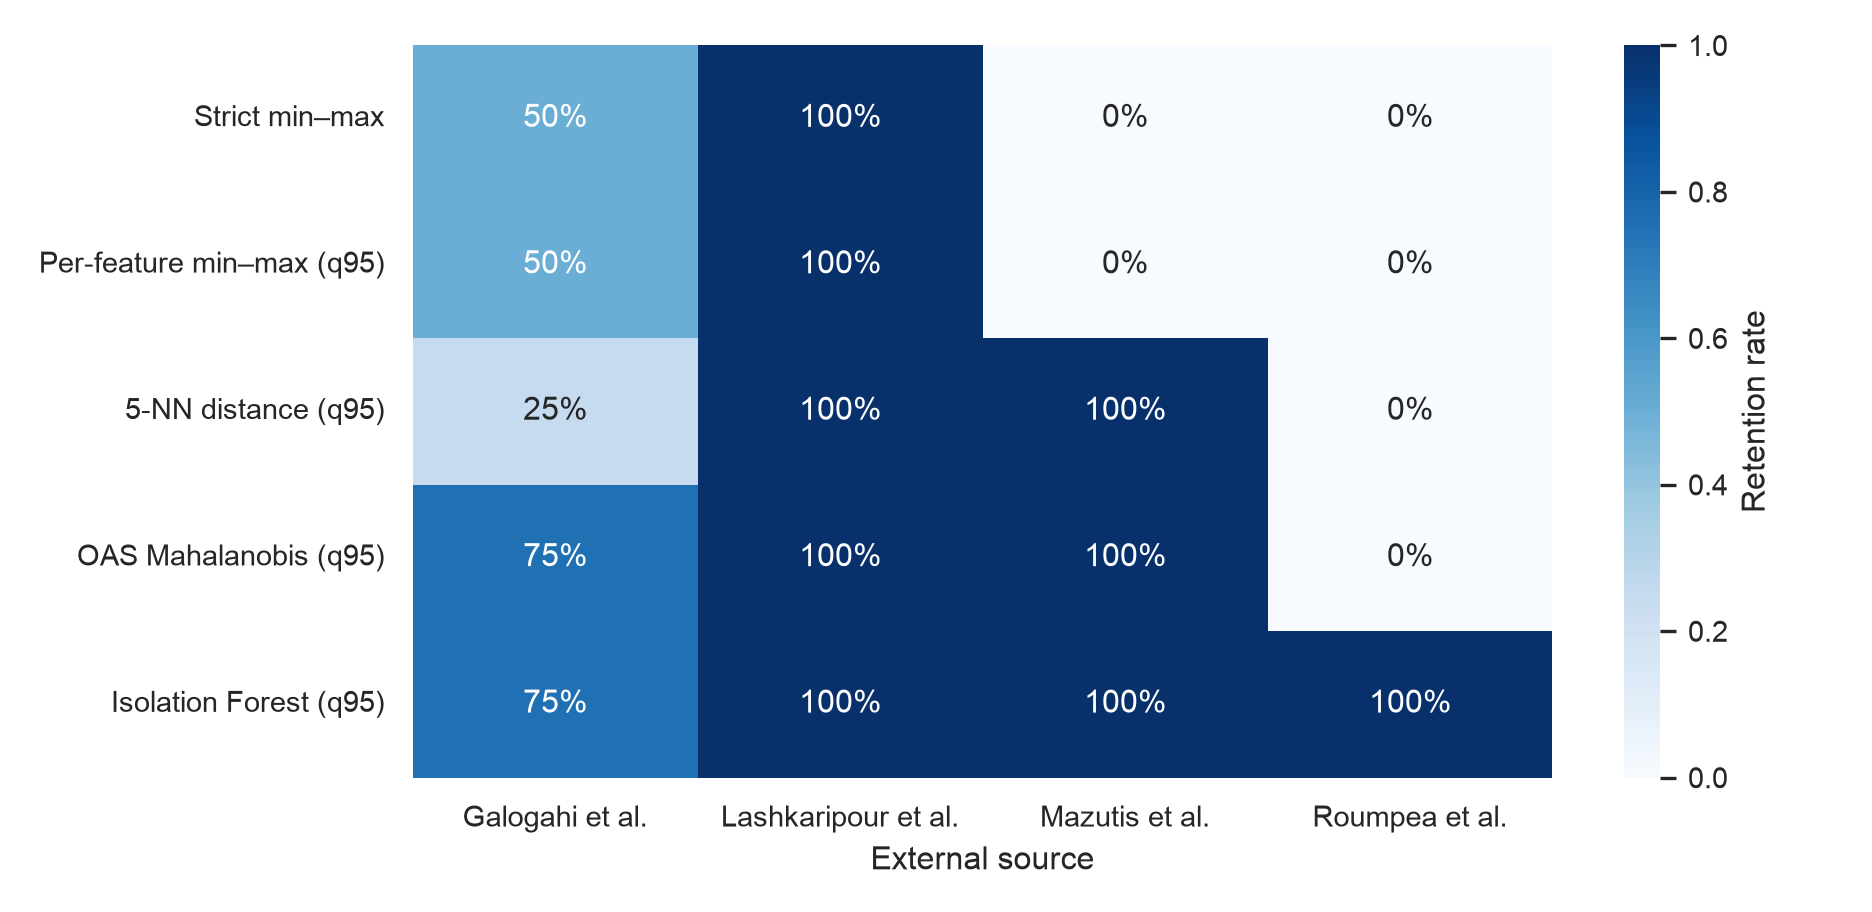
\includegraphics[width=0.85\linewidth]{expanded_figure_4_source_retention}
\caption{95\% 校准分位数下二值规则按外部来源的保留率。每条规则的保留都按来源分块,这就是来源内上下文置换零分布能够解释所观察到的风险降低的原因。}
\label{fig:retention}
\end{figure}

\subsection{R8:跨偏移单元的方法矩阵基准}
\label{sec:r8}

冻结矩阵协议(第~\ref{sec:w3protocol}~节)的两次完整运行在不同目录中产生了逐字节相同的产物哈希清单(各 13 项),且全部 69 个单元–重复划分(覆盖七个单元)在拟合、校准与测试行之间的依赖单元重叠均为零。表~\ref{tab:w3matrix} 给出参考 XGBoost 模型、两个替代点模型和四种区间方法的矩阵。由于点模型只看到拟合分区,参考单元高于第~\ref{sec:r1}~节的 E0 误差(D1 为 6.71\% 对 5.27\%);表中的比值是本协议内部的量。

\begin{table}[t]
\centering\small
\caption{方法矩阵基准。XGBoost MAPE 及其相对于数据集随机划分参考的比值、替代点模型,以及名义 90\% 区间的经验覆盖率(XGBoost;各重复的均值)。参考单元使用拟合分区,不可与表~\ref{tab:repro} 比较。}
\label{tab:w3matrix}
\resizebox{\linewidth}{!}{%
\begin{tabular}{llrrrrrrrrr}
\toprule
单元 & 偏移 & 重复次数 & XGB & 比值 & RF & MLP & 分割共形 & CQR & Mondrian & 集成方差 \\
\midrule
D1 随机 & 参考 & 15 & 6.71\% & 1.00 & 6.86\% & 14.52\% & 0.959 & 0.948 & 0.998 & 0.917 \\
D1 几何 & 器件几何 & 30 & 12.43\% & 1.85 & 11.78\% & 55.67\% & 0.860 & 0.866 & 0.970 & 0.854 \\
D1 外部 & 跨文献 & 1 & 11.66\% & 1.74 & 11.80\% & 16.70\% & 0.453 & 0.484 & 0.734 & 0.547 \\
D1 SE$\to$DE & 器件类型 & 1 & 22.12\% & 3.30 & 21.19\% & 266.34\% & 0.330 & 0.414 & 0.525 & 0.586 \\
D1 DE$\to$SE & 器件类型 & 1 & 69.18\% & 10.31 & 73.67\% & 3592.49\% & 0.065 & 0.051 & 0.097 & 0.259 \\
D2 随机 & 参考 & 15 & 3.91\% & 1.00 & 5.32\% & 5.35\% & 0.904 & 0.911 & 0.989 & 0.891 \\
D2 化学体系 LOCO & 全化学体系 & 6 & 10.24\% & 2.62 & 9.07\% & 21.16\% & 0.528 & 0.786 & 0.857 & 0.670 \\
\bottomrule
\end{tabular}}
\end{table}

\begin{table}[t]
\centering\small
\caption{方法矩阵基准。每种适用域得分与对照的相对误差风险—覆盖曲线 AURC(越低越好),XGBoost,各重复的均值;粗体标出每个单元中的最佳项。}
\label{tab:w3aurc}
\resizebox{\linewidth}{!}{%
\begin{tabular}{lrrrrrrrr}
\toprule
单元 & 全池 & 随机 & 仅尺寸 & 5-NN & 马氏距离 & 孤立森林 & 域分类器 & 密度比 \\
\midrule
D1 随机 & 0.0671 & 0.0662 & 0.0541 & \textbf{0.0466} & 0.0516 & 0.0535 & 0.0653 & 0.0543 \\
D1 几何 & 0.1243 & 0.1255 & 0.1141 & \textbf{0.1085} & 0.1142 & 0.1225 & 0.1153 & 0.1097 \\
D1 外部 & 0.1166 & 0.1107 & \textbf{0.0913} & 0.1135 & 0.0957 & 0.1178 & 0.1161 & 0.1039 \\
D1 SE$\to$DE & 0.2212 & 0.2256 & 0.3128 & 0.1442 & 0.1467 & 0.2219 & \textbf{0.1394} & 0.1737 \\
D1 DE$\to$SE & 0.6918 & 0.6734 & 0.6423 & 0.6017 & 0.5874 & \textbf{0.4182} & 0.5729 & 0.5263 \\
D2 随机 & 0.0391 & 0.0388 & 0.0398 & 0.0365 & 0.0379 & 0.0371 & 0.0368 & \textbf{0.0324} \\
D2 化学体系 LOCO & 0.1024 & 0.1102 & 0.0884 & 0.0893 & 0.1089 & \textbf{0.0816} & 0.1013 & 0.1036 \\
\bottomrule
\end{tabular}}
\end{table}

\paragraph{器件类型偏移是这些数据中最大的偏移} 以 474 个单乳液行训练、394 个双乳液行测试,XGBoost MAPE 升至 22.12\%(相对 D1 参考的比值为 3.30);反方向给出 69.18\%(比值 10.31)。几何分组(12.43\%,比值 1.85)、跨文献迁移(11.66\%,1.74)和 D2 上的全化学体系留一(10.24\%,2.62)均较小。随机森林在每个单元中都与 XGBoost 接近(器件类型偏移下为 21.19\% 和 73.67\%)。固定架构的多层感知机(其早停在每次拟合中均在 75–696 次迭代内触发)在器件类型偏移下外推至 266.34\% 和 3592.49\%,在几何分组下为 55.67\%:一个无界回归器一旦离开训练支撑,就没有任何东西能把它约束在物理范围之内。该矩阵还在除拟合分区差异之外复现了第~\ref{sec:r2}、\ref{sec:r5}和\ref{sec:r6}~节的量:留一化学体系单元的 TX100 折给出 20.75\%($n=87$,带符号相对偏差 0.203),而密封结果为 19.84\%;其余五折的范围为 5.22\% 至 16.15\%;六折宏平均为 10.24\%,B1 为 10.27\%;外部单元为 11.66\%(Galogahi 7.71\%,Lashkaripour 9.03\%,Mazutis 17.87\%,Roumpea 19.52\%;来源宏平均 13.53\%),868 行模型为 11.26\%。

\paragraph{区间迁移} 在参考单元上,三种行级方法接近名义水平(D1:分割共形 0.959,CQR 0.948,集成方差 0.917;D2:0.904,0.911,0.891),而组最大值 Mondrian 共形过度覆盖(0.998,0.989)。在几何分组下,行级方法降至 0.854–0.866,而 Mondrian 的行级经验覆盖率达到 0.970,平均宽度为 78.4 µm(分割共形为 43.9 µm);不过由于校准组很少,其组级有限样本保证的可达上限只有 0.857,低于 90\% 的目标。在跨文献偏移下,覆盖率为 0.453(分割)、0.484(CQR)、0.547(集成)和 0.734(Mondrian,36.8 µm 对 26.3 µm)。在全化学体系留一下,CQR 保持 0.786,而分割共形为 0.528,集成方差为 0.670;Mondrian 仅靠扩宽至 87.2 µm(对 21.6 µm)才达到 0.857。在器件类型偏移下,每个在训练器件类型内校准的区间都近乎失效(SE$\to$DE 为 0.330–0.586;DE$\to$SE 为 0.051–0.259)。

\paragraph{适用域得分与对照} 表~\ref{tab:w3aurc} 给出每个单元中每种得分与对照的 AURC。跨文献单元复现了第~\ref{sec:r7}~节:仅尺寸对照(0.0913)优于每一种适用域得分,最接近的是马氏距离(0.0957)。在器件类型偏移下情形反转——仅尺寸对照比随机更差(SE$\to$DE 为 0.3128 对 0.2256),而域分类器(domain classifier,0.1394)、5-NN(0.1442)和马氏距离(0.1467)远低于全池风险 0.2212——因此液滴尺寸不是器件类型变化的代理。以 0.95 校准分位数为阈值的二值规则几乎不保留任何双乳液行(两个方向的 5-NN 保留率均为 0.000;孤立森林在 SE$\to$DE 为 0.023,精度 1.000,10 µm 处召回率 0.043)。这正是我们自己偏差登记册中已有警告的形式化对应:第~\ref{sec:r4}~节的规范剪枝阈值是在单乳液行上校准的,不支持关于双乳液候选的任何声明。在全化学体系留一下,全局 5-NN 规则降低了精度(10 µm 处为 0.416,而全池率为 0.514;保留率 0.785,召回率 0.824),而孤立森林提高了精度(0.541;保留率 0.894,召回率 0.945):靠近训练化学体系并不等同于在新化学体系上可靠。在跨文献单元中,5-NN 规则保留 0.688 的行,精度 0.886,召回率 0.975,而拟合分区模型的全池率为 0.625。

\paragraph{候选级规则} 预先登记的组内判据在跨文献单元中没有任何得分满足(5 个得分中 0 个),与第~\ref{sec:r7}~节一致。在几何分组单元中,转导式(transductive)域分类器在 30 个种子中的 12 个满足它(组内 AURC 0.1126,随机为 0.1238,仅尺寸为 0.1244),5-NN 为 1 个,马氏距离 2 个,密度比 3 个,孤立森林 0 个;域分类器看到测试输入,因此描述的是批量筛选,而非逐候选到达。在两个参考单元中,该判据在每个得分的 15 个种子中触发 1–2 个,与 5\% 假阳性率处于同一量级。尽管器件类型单元在名义上通过了组内检验,这些通过在实际上是空洞的:SE$\to$DE 只有 2 个测试组,而在 DE$\to$SE(35 组)中参考模型本身已经失败(全池风险 0.6918),因此组内排序所排列的是一个失败的模型。留一化学体系单元每折只有一个测试组,在该判据下不可评估。

\paragraph{度量稳健性与尺寸混杂(事后)} 两个器件类型单元是单次固定划分,因此其不确定性针对行而非种子:XGBoost MAPE 的行自助法 95\% 区间为 20.66–23.56\%(SE$\to$DE)、65.38–73.28\%(DE$\to$SE)和 9.75–13.62\%(跨文献)。表~\ref{tab:w3robust} 在中位 APE、对称 MAPE 和绝对对数比误差下重新计算每个单元。五个偏移单元按相对参考单元比值的排序在 MAPE、对称 MAPE 和对数比误差下相同(DE$\to$SE、SE$\to$DE、全化学体系、几何、跨文献);在中位 APE 下,跨文献单元(2.89)移到化学体系(2.66)和几何(2.21)之上,两个器件类型单元仍居首位(15.02 和 4.92)。器件类型与液滴尺寸相混杂:单乳液行的观测直径为 28.11–245.1 µm(中位数 85.71),双乳液行为 15.57–54.21 µm(中位数 35.12);0.698 的双乳液行位于单乳液尺寸范围内,而只有 0.141 的单乳液行位于双乳液范围内。尺寸四分位分箱显示,误差并不局限于范围外的尺寸。对于 SE$\to$DE,MAPE 随液滴尺寸上升——6.43\%(15.6–27.2 µm,$n=99$)、12.78\%(27.2–35.1 µm)、33.02\%(35.1–40.6 µm)和 36.25\%(40.6–54.2 µm)——因此最大的误差落在其尺寸被单乳液训练集覆盖的双乳液行上。对于 DE$\to$SE,与双乳液范围重叠的最小单乳液四分位(28.1–63.3 µm,$n=119$)的 MAPE 最高,为 104.20\%,较大的四分位依次降至 77.90\%(63.3–85.7 µm,$n=118$)、61.46\%(85.7–118.3 µm,$n=118$)和 33.15\%(118.3–245.1 µm,$n=119$)。因此,器件类型偏移既在重叠的尺寸范围内、也在其范围之外使预测变差。

\begin{table}[t]
\centering\small
\caption{方法矩阵的事后度量稳健性(XGBoost;各重复的均值;不属于冻结协议)。中位 APE 与对称 MAPE 以百分数给出;对数比误差为 $\log(\hat d/d)$ 的平均绝对值。比值是相对于同一数据集随机划分参考单元、在同一度量下计算的。}
\label{tab:w3robust}
\resizebox{\linewidth}{!}{%
\begin{tabular}{lrrrrrr}
\toprule
单元 & MdAPE & sMAPE & 对数比 & MdAPE 比值 & sMAPE 比值 & 对数比比值 \\
\midrule
D1 随机 & 4.39\% & 6.80\% & 0.068 & 1.00 & 1.00 & 1.00 \\
D1 几何 & 9.71\% & 12.45\% & 0.125 & 2.21 & 1.83 & 1.84 \\
D1 外部 & 12.69\% & 11.66\% & 0.117 & 2.89 & 1.71 & 1.71 \\
D1 SE$\to$DE & 21.60\% & 25.89\% & 0.263 & 4.92 & 3.81 & 3.85 \\
D1 DE$\to$SE & 65.92\% & 47.47\% & 0.492 & 15.02 & 6.98 & 7.20 \\
D2 随机 & 2.88\% & 3.83\% & 0.038 & 1.00 & 1.00 & 1.00 \\
D2 化学体系 LOCO & 7.69\% & 10.21\% & 0.103 & 2.66 & 2.67 & 2.69 \\
\bottomrule
\end{tabular}}
\end{table}

\paragraph{不确定性感知模型族:点误差与偏移排序} 表~\ref{tab:w4} 报告第~\ref{sec:w4protocol}~节的分位数森林、高斯过程和深度集成在相同单元、种子和分区上的结果,来自两次具有逐字节相同的 11 项清单的运行。偏移排序是数据的属性而非 XGBoost 的属性:对每个模型族,DE$\to$SE 单元相对其自身参考的误差比值最大(9.37、8.93 和 226.33),SE$\to$DE 对森林和过程居第二(2.77 和 3.96)。深度集成与矩阵中的单个感知机一样,在器件类型偏移下爆炸(302.83\% 和 3271.87\%)。

\paragraph{不确定性感知模型族:区间覆盖率与高斯过程的例外} 没有任何在训练器件类型内校准的区间在 DE$\to$SE 方向上保持覆盖:原生覆盖率为 0.072(森林)、0.652(过程)和 0.000(集成),而共形化无济于事(0.072、0.629、0.000)。与"没有任何原生区间能在任一器件类型单元中存活"这一预先登记预期唯一不符的,是高斯过程在 SE$\to$DE 中的表现:其原生区间覆盖了 0.959 的双乳液行(共形化后为 0.982),因为其预测标准差在训练支撑之外增长——平均宽度为 49.2 µm,而森林为 9.7 µm,所针对的行其直径中位数为 35.12 µm;同一机制在相反方向上失败(宽度 162.0 µm 时为 0.652)。在全化学体系偏移下,森林的原生区间达到 0.830(宽度 51.4 µm),高于矩阵中 CQR 的 0.786,并且是两个协议中任何区间的最高覆盖率;在跨文献偏移下,共形化森林达到 0.812,共形化集成在 84.2 µm 处达到 0.906,而 XGBoost 分割共形区间仅覆盖 0.453。共形化在三个模型族的两个参考单元上都恢复了近名义覆盖率(D1 上为 0.903–0.953,D2 上为 0.894–0.896;过程对 D1 过度覆盖,为 0.953,略微超出预先登记的 0.05 带),而深度集成的原生区间即使在分布内也严重欠分散(0.403 和 0.535),这是没有似然头的均值—方差集成的已知行为。

\paragraph{不确定性感知模型族:原生不确定性作为得分} 模型原生不确定性是良好的分布内排序得分——对森林和过程,它在 D1 随机划分重复的 0.93 中同时优于两种对照——但正如预先登记的预期所料,每个模型族在至少一个偏移单元中被仅尺寸对照或随机得分击败:森林的分位间隔在 SE$\to$DE 中对双乳液候选的排序比随机更差(0.3072 对 0.2132),并在跨文献单元中被仅尺寸击败(0.1115 对 0.0994);过程在两个器件类型单元中均被仅尺寸击败(0.3760 对 0.3145;0.8487 对 0.7968);集成的得分在 DE$\to$SE 中失败。因此,矩阵的区间发现并非 XGBoost 特有:崩溃是偏移的属性,唯一的限定是,不确定性随到训练输入的距离增长的模型,可以在器件类型偏移的某一方向上,通过将区间扩宽至与其所预测的量同一尺度来换取覆盖率。

\begin{table}[t]
\centering\small
\caption{方法矩阵单元上的不确定性感知模型族(冻结的 W4 协议;各重复的均值;两次运行逐字节相同)。比值为 MAPE 相对于同一模型随机划分参考单元的比。名义 90\% 区间的覆盖率:原生、围绕点预测的分割共形,以及共形化后的原生区间。各模型自身的相对误差风险—覆盖曲线的 AURC(越低越好):分别针对该模型的相对不确定性得分和仅尺寸对照。}
\label{tab:w4}
\resizebox{\linewidth}{!}{%
\begin{tabular}{llrrrrrrr}
\toprule
单元 & 模型 & MAPE & 比值 & 原生 & 分割 & 共形化 & AURC 不确定性 & AURC 仅尺寸 \\
\midrule
D1 随机 & QRF & 7.65\% & 1.00 & 0.908 & 0.947 & 0.903 & 0.0540 & 0.0622 \\
 & GP & 9.51\% & 1.00 & 0.860 & 0.974 & 0.953 & 0.0596 & 0.0679 \\
 & 深度集成 & 14.46\% & 1.00 & 0.403 & 0.960 & 0.914 & 0.0784 & 0.1065 \\
D1 几何 & QRF & 12.00\% & 1.57 & 0.859 & 0.863 & 0.873 & 0.1047 & 0.1115 \\
 & GP & 20.81\% & 2.19 & 0.709 & 0.862 & 0.885 & 0.1847 & 0.1907 \\
 & 深度集成 & 39.81\% & 2.75 & 0.608 & 0.847 & 0.885 & 0.3328 & 0.3838 \\
D1 外部 & QRF & 11.95\% & 1.56 & 0.781 & 0.531 & 0.812 & 0.1115 & 0.0994 \\
 & GP & 20.51\% & 2.16 & 0.734 & 0.625 & 0.734 & 0.1500 & 0.2180 \\
 & 深度集成 & 17.80\% & 1.23 & 0.328 & 0.906 & 0.906 & 0.1202 & 0.1226 \\
D1 SE$\to$DE & QRF & 21.18\% & 2.77 & 0.525 & 0.411 & 0.525 & 0.3072 & 0.3064 \\
 & GP & 37.60\% & 3.96 & 0.959 & 0.122 & 0.982 & 0.3760 & 0.3145 \\
 & 深度集成 & 302.83\% & 20.95 & 0.330 & 0.030 & 0.391 & 1.4859 & 4.5986 \\
D1 DE$\to$SE & QRF & 71.65\% & 9.37 & 0.072 & 0.044 & 0.072 & 0.5954 & 0.6664 \\
 & GP & 84.87\% & 8.93 & 0.652 & 0.017 & 0.629 & 0.8487 & 0.7968 \\
 & 深度集成 & 3271.87\% & 226.33 & 0.000 & 0.000 & 0.000 & 35.0508 & 32.0161 \\
D2 随机 & QRF & 6.39\% & 1.00 & 0.928 & 0.907 & 0.894 & 0.0532 & 0.0636 \\
 & GP & 3.65\% & 1.00 & 0.884 & 0.899 & 0.896 & 0.0332 & 0.0364 \\
 & 深度集成 & 5.12\% & 1.00 & 0.535 & 0.894 & 0.896 & 0.0417 & 0.0522 \\
D2 化学体系 LOCO & QRF & 9.85\% & 1.54 & 0.830 & 0.702 & 0.758 & 0.0825 & 0.0967 \\
 & GP & 16.60\% & 4.55 & 0.699 & 0.359 & 0.716 & 0.1382 & 0.1333 \\
 & 深度集成 & 20.89\% & 4.08 & 0.274 & 0.359 & 0.447 & 0.1751 & 0.1877 \\
\bottomrule
\end{tabular}}
\end{table}

\paragraph{协变量偏移加权不能挽救区间} 表~\ref{tab:w5} 报告参考 XGBoost 模型在第~\ref{sec:w5protocol}~节中的重加权分割共形区间(两次运行,逐字节相同的 7 项清单;未加权分支在全部 69 个单元–重复划分上以机器精度复现矩阵的分割共形覆盖率)。在参考单元上,域分类器权重保持接近 1,使覆盖率至多移动 0.005(D1 上 0.959 到 0.955,D2 上 0.904 到 0.899),符合预期。$k$-NN 密度比在八维中过于粗糙——即便在分布内其有效样本量也仅为校准集的 0.137——并使 D1 覆盖率降至 0.863,超出预先登记的 0.03 带。在器件类型和跨文献偏移下,两种加权都使每个测试权重比校准权重高出若干数量级,因此每个区间都变为无穷:所报告的覆盖率 1.000 是弃权,而非预测,不存在有限区间覆盖率。当测试输入位于校准支撑之外时,这正是该方法的正确行为,且与不保留任何双乳液行的适用域筛选相吻合;这也意味着,恰恰在覆盖率丢失的单元中,协变量偏移修复无能为力。在几何偏移(此处最温和的偏移)下,域加权恢复了名义覆盖率(0.908 对 0.860),代价是 0.209 的区间为无穷,有限区间为 52.1 µm,而未加权为 43.9 µm。在全化学体系偏移下,它达到 0.848(对 0.528),但 0.326 的区间为无穷,有限区间在 77.5 µm 处仅覆盖 0.662(未加权为 21.6 µm);按预先声明的覆盖率终点,域加权在 6 折中的 4 折上存活,多于预先登记的预期所允许的,而且这主要靠弃权实现(在 TX100 折上,约四分之三的区间为无穷)。因此,化学体系失败无法通过任何仅依赖输入的重加权修复,这与对 TX100 结果的条件偏移解读一致,而器件类型失败是一种支撑不匹配,重加权可以指认但无法修复。

\begin{table}[t]
\centering\small
\caption{参考 XGBoost 模型的协变量偏移加权分割共形(冻结的 W5 协议;各重复的均值;两次运行逐字节相同)。“Cov.”将无穷区间计为覆盖;“inf.”为无穷区间所占比例;“fin. cov.”与“width”仅针对有限区间;ESS 为校准权重的有效样本量除以校准集大小。破折号:每个区间均为无穷。列分组:未加权;域分类器几率(Domain-classifier odds);$k$-NN 密度比。}
\label{tab:w5}
\resizebox{\linewidth}{!}{%
\begin{tabular}{lrr|rrrrr|rrrrr}
\toprule
 & \multicolumn{2}{c|}{未加权} & \multicolumn{5}{c|}{域分类器几率} & \multicolumn{5}{c}{$k$-NN 密度比} \\
单元 & 覆盖 & 宽度 & 覆盖 & 无穷 & 有限覆盖 & 宽度 & ESS & 覆盖 & 无穷 & 有限覆盖 & 宽度 & ESS \\
\midrule
D1 随机 & 0.959 & 33.0 & 0.955 & 0.000 & 0.955 & 32.4 & 0.841 & 0.863 & 0.002 & 0.862 & 24.1 & 0.137 \\
D1 几何 & 0.860 & 43.9 & 0.908 & 0.209 & 0.880 & 52.1 & 0.420 & 0.886 & 0.553 & 0.788 & 42.0 & 0.168 \\
D1 外部 & 0.453 & 26.3 & 1.000 & 1.000 & — & — & 0.076 & 1.000 & 1.000 & — & — & 0.281 \\
D1 SE$\to$DE & 0.330 & 8.9 & 1.000 & 1.000 & — & — & 0.998 & 1.000 & 1.000 & — & — & 0.416 \\
D1 DE$\to$SE & 0.065 & 21.2 & 1.000 & 1.000 & — & — & 0.836 & 1.000 & 1.000 & — & — & 0.018 \\
D2 随机 & 0.904 & 23.8 & 0.899 & 0.000 & 0.899 & 23.7 & 0.963 & 0.917 & 0.004 & 0.917 & 26.7 & 0.431 \\
D2 化学体系 LOCO & 0.528 & 21.6 & 0.848 & 0.326 & 0.662 & 77.5 & 0.243 & 0.852 & 0.568 & 0.546 & 37.6 & 0.151 \\
\bottomrule
\end{tabular}}
\end{table}

\subsection{R9:实验室偏移下的第二次密封验证——负结果}
\label{sec:r9}

Smart Microfluidics 密封集的揭盲闸门被消耗了一次(2026-10-17T03:41:48Z),此前揭盲程序已重新核验协议、绑定、偏差登记册、保管人清单、预测包和三个冻结程序文件的摘要。表~\ref{tab:d3} 列出锁定的终点。在 246 个实验室 A 行上拟合的冻结 XGBoost 尺寸代理模型,在 57 个密封的实验室 B 行上的 MAPE 为 240.39\%,而冻结的开发参照为 39.41\%(复现阈值 49.27\%);两项预先声明的判据均未满足。没有密封行(0/57,比例 0.000)的相对误差在 10\% 以内;中位绝对百分比误差(MdAPE,描述性)为 206.74\%,MAE 为 595.3 nm,RMSE 为 1335.0 nm,$R^2=0.026$,带符号相对偏差为 $-0.700$,被高估的行占 0.456。名义 90\% 分割共形区间(校准半径 344.19 nm,来自 50 个校准行;196 个拟合行)覆盖了 0.719 的行,平均宽度为 688.4 nm。观测尺寸的中位数为 98.8 nm(范围 64.4–7932.7 nm);预测值的中位数为 200.0 nm,但范围从 $-336.3$ 到 4036.1 nm:57 个点预测中有 22 个(38.6\%)是负直径,57 个区间下界中有 46 个(80.7\%)小于或等于零。冻结配置中没有任何东西约束输出,而这些行在物理上是不可能的。

\paragraph{失败原因(Why it failed)} 在任何拟合之前,输入侧已有两项事实在案(第~\ref{sec:d3protocol}~节):每个实验室 B 行都使用 PBS 缓冲液,而开发集有 231 个 MQ 行和 15 个 PBS 行;并且 57 行中仅 18 行(31.6\%)落在逐特征开发范围之内(PEG 支撑比例 0.316,HSPC 0.684)。揭盲后,18 个范围内行的中位绝对相对误差为 0.884,39 个范围外行为 2.755。因此范围违反与误差强相关,但边际范围内 88\% 的中位误差,如同 TX100 一样,也是一种条件偏移:同样的 PBS 配方在另一实验室的设备上给出不同的尺寸。与 TX100 情形不同,边际筛选在揭盲前确实标出了问题;它们做不到的是把被标出的批次转变为可靠的候选。

\paragraph{适用域规则(Applicability rules)} 在修正后的适用域块(第~\ref{sec:d3protocol}~节)中,全池平均绝对相对误差为 2.404,在任何规则下可靠行(10\% 以内)的数量均为零。0.95 分位数处的 5-NN 规则保留 57 行中的 7 行(0.123),保留风险为 1.079,等预算随机 $p=0.0046$,四条规则间 BH 校正 $p=0.018$;它在形式上满足四项锁定条件,但可靠候选为零,且面对一个保留 57 行中 23 行(0.404)、风险 1.204 的仅预测尺寸对照($p=0.0001$),我们不作任何收益声明。马氏距离保留 2 行(风险 1.295,$p=0.169$,BH 0.225),域分类器 1 行(0.237,$p=0.053$,BH 0.106),孤立森林无(0/57),严格 min–max 18 行(1.614,$p=0.0027$)。在候选层面,预先登记的缓冲液分层不可评估(密封集中只有一个水平);在修订后的主脂质(main-lipid)分层(ESM 27,HSPC 30)下,所有四个得分都优于随机对照(分层内 AURC 2.105):5-NN 1.926($p=0.0025$,BH 0.0033),马氏距离 1.850($p=0.0005$,BH 0.0010),孤立森林 2.023($p=0.016$),域分类器 1.806($p=0.0005$)。没有一个优于仅预测尺寸对照(1.562),因此裁决是没有候选级收益,与第~\ref{sec:r7}和\ref{sec:r8}~节一致。

\paragraph{其他度量与对数目标基线(事后)} 头条 MAPE 不是尾部伪影:在同样的 57 行上,对称 MAPE 为 129.60\%,中位 APE 为 206.74\%,35 个正预测上的平均绝对对数比误差为 0.969;观测尺寸的每个四分位都带有大误差和部分负预测(MAPE 249.9\%、306.5\%、241.1\% 和 169.1\%,中位 APE 208.7\%、402.4\%、201.6\% 和 102.6\%,对应尺寸 64.4–92.9、92.9–98.8、98.8–130.2 和 130.2–7932.7 nm,负预测比例 0.286、0.571、0.357 和 0.333;$n=14$、14、14 和 15)。将锁定配置重新拟合到 $\log(\mathrm{size})$ 改变了局面。其分组五折开发参照为 16.89\%,而原尺度模型为 39.41\%(重新拟合精确复现了后者的折和预测),因此原尺度目标在实验室 A 内部就已代价高昂。在实验室 B 上,对数目标模型给出 MAPE 43.05\%,中位 APE 34.57\%,对称 MAPE 52.94\%,平均绝对对数比 0.644,10\% 以内的行占 0.070,且没有负预测;其预测跨越 56.5–366.3 nm,而观测尺寸高达 7932.7 nm,其最大尺寸四分位仍然最差(65.8\%,较小的四分位分别为 38.7\%、25.8\% 和 40.2\%)。该 43.05\% 低于冻结的复现阈值 49.27\%,但为该模型自身开发参照的 2.55 倍(阈值 21.11\%),因此未满足同口径(like-for-like)判据。我们将冻结结果解读为两个可分离的成分:继承自已发表配置的目标尺度选择,它产生了负预测和大部分量级;以及约为开发误差两倍半的残余实验室偏移,它在修正后依然存在。由于对数目标模型是在揭盲后选定的,它是一种诊断,而非验证结果。

\paragraph{次要终点(Secondary endpoints)} 多分散指数(PDI)的预测 MAPE 为 41.24\%(MdAPE 31.44\%;10\% 以内的行占 0.105)。形成分类器(formation classifier)的准确率为 0.912,F1 为 0.954,但 57 个密封行中有 53 个为正,因此多数类基线为 0.930,分类器并未超过它。12 行的次要密封集(操作者 B,实验室 A,同一设备)不属于主要估计目标,仅作描述性报告,给出 MAPE 220.27\%,MdAPE 71.87\%,10\% 以内的行占 0.25,覆盖率 0.833,以及 3/12 个负预测;操作者偏移下的中位误差远低于实验室偏移下的,但 12 行不足以支撑更强的论断。

\paragraph{披露(Disclosure)} 揭盲后发现,冻结揭盲程序的适用域收益块接收的是带符号而非绝对的相对误差,这就是冻结结果文件显示全池“风险”为 $-0.700$ 的原因。主要终点、两项判据、区间块、候选级块以及每个点指标均使用绝对误差,不受影响。该块由另一个程序在已揭盲的行上重新计算并写入单独文件;没有任何冻结产物被修改。我们将 D3 揭盲描述为*一次密封预测,随后是对适用域块的一次已披露的揭盲后评分修正*。闸门已被消耗:实验室 B 和操作者 B 的标签不再是盲的,对它们的任何进一步分析均为回顾性的。

\begin{table}[t]
\centering\small
\caption{第二次密封验证的锁定终点(Smart Microfluidics,实验室 A $\to$ 实验室 B,$n=57$)。}
\label{tab:d3}
\resizebox{\linewidth}{!}{%
\begin{tabular}{lr}
\toprule
终点 & 值 \\
\midrule
开发参照 MAPE(实验室 A,分组五折交叉验证,揭盲前冻结) & 39.41\% \\
复现($\le 1.25\times$)/ 强复制($\le 1.00\times$)阈值 & 49.27\% / 39.41\% \\
密封实验室 B MAPE & 240.39\% \\
复现 / 强复制判据 & 未满足 / 未满足 \\
MdAPE(描述性) & 206.74\% \\
MAE / RMSE & 595.3 / 1335.0 nm \\
$R^2$ & 0.026 \\
相对误差 10\% 以内的行 & 0/57 (0.000) \\
带符号相对偏差 / 被高估比例 & $-0.700$ / 0.456 \\
名义 90\% 覆盖率(平均宽度) & 0.719 (688.4 nm) \\
负点预测 & 22/57 (38.6\%) \\
区间下界 $\le 0$ & 46/57 (80.7\%) \\
严格 min–max 接受(揭盲前记录) & 18/57 (31.6\%) \\
候选级收益(主脂质分层) & 无:4 个得分中 4 个优于随机,4 个得分中 0 个优于仅尺寸 \\
\bottomrule
\end{tabular}}
\end{table}

\section{讨论}
\label{sec:discussion}

\paragraph{证据所支持的结论} 公开的实验表格可以训练出有用的微流控代理模型(surrogate)(R1)。在跨文献、跨器件和跨化学体系的偏移(shift)下,随机划分的测试集低估了部署风险(R2、R5、R7)。在可交换(exchangeable)行上校准得到的名义共形覆盖(conformal coverage)无法迁移到发生偏移的数据来源,而分组校准只能以较大的区间宽度为代价恢复覆盖率(R3、R7)。无标签筛选(label-free screen)可以提高被保留候选的成功率,但同时损失召回率;在这些数据上,这种增益体现在文献来源的层面(R4、R7)。在留一化学体系(leave-one-chemistry-out)评估下,冻结的物理引导硬约束回归器并未改善宏平均误差,但硬边界消除了物理上无效的输出(R6)。在由七个单元构成的方法矩阵中,单乳液与双乳液之间的器件类型偏移(device-type shift)比几何、文献或化学体系偏移更严重地恶化误差;在一种器件类型上校准的无标签筛选,在另一种器件类型上几乎什么都留不住;在整体化学体系偏移下,分位数回归区间比对称残差区间更好地维持了覆盖率(R8)。在独立脂质体数据集上、于实验室偏移(laboratory shift)下进行的第二次密封测试(sealed test)大幅失败,并且由一个无边界的代理模型产生了负的直径,而协变量支持域缺口(covariate-support gap)在揭示(reveal)之前仅凭输入即可看出(R9)。

\paragraph{证据不支持的结论} 没有任何材料、配方、器件或操作路径被证明在湿实验中可行;我们也不主张化学相容性、可制造性、稳定滴落(dripping)或前瞻性发现。共形覆盖对任何新的化学体系或器件均无保证。TX100 的负面结果只是针对一个数据集、一个采用已发表特征的基线所做的一次密封测试,并不代表机器学习的普遍失败。此处没有任何适用性(applicability)规则是最终的或最优的剪枝算法,也没有任何一条被证明能在单一来源内部的候选层面起作用。第二次密封结果对应的是一个冻结配置(实验室 A 的数据、V1 的 XGBoost 配置),处于一种与缓冲液(buffer)相混淆的双实验室偏移之下;它不是对 Smart Microfluidics 数据集或其作者所建模型的评估,对配方质量或临床相关性也不构成任何说明。转导式(transductive)域分类器在几何偏移下的候选级通过(30 个种子中的 12 个)是在手握测试输入的情况下做出的批量筛选观察,并不保证对逐个到达的候选同样成立。

\paragraph{密封带来了什么} 密封的 TX100 误差(19.84\%)与同一组上回顾性的留一化学体系折(20.75\%)相当,其余五折介于 5.22\% 与 16.15\% 之间;交叉验证本可以得到同样量级的结果。密封并未使失败比这更大或更出人意料,我们也不将其如此呈现。它所增加的东西更为有限:模型、终点和决策规则在看到任何标签之前即已固定,因此这一负面结果不可能是在留出组上调参的残余;该估计是前瞻性的而非经过挑选的;时间顺序是可审计的。与回顾性折相吻合,说明的是密封数值具有代表性,而不是说密封可有可无。D3 亦然:事后的对数目标变换重拟合表明冻结结果中有多大一部分源于建模选择——而这种选择之所以看得清楚,恰恰是因为它在结果已知之前就已固定。

\paragraph{九项结果合起来说明了什么} 综合来看,这些结果支持六点观察,其中任何单一结果都无法独自确立。第一,在这些数据之内,各类偏移按严重程度排序:按行随机划分与完全相同输入的划分几乎可互换;几何分组与跨文献迁移使参考误差乘以 1.74--1.85;整体化学体系留出为 2.62;器件类型偏移为 3.30 和 10.31;跨实验室的脂质体测试则远高于其自身的开发参考值(表~\ref{tab:d3})。第二,失败分为两层,需要不同的检测手段:一层是支持域缺口,边缘分布筛选仅凭输入即可看出(D3:PEG 与 HSPC 的支持域占比分别为 0.316 与 0.684);另一层是条件偏移(conditional shift),它们看不出来(TX100:每一行都在范围之内;D3:即使在边缘范围之内,中位误差也为 0.884)。只有第一层可以在无标签的条件下处理;第二层要么需要未被记录的状态变量,要么需要来自目标域的标签。第三,恰当的负对照取决于偏移的类型:在跨文献和跨实验室偏移下,尺寸代理(size proxy)的排序优于每一种适用性评分,但在器件类型偏移下反而不如随机,因此每当主张适用性带来收益时,两种对照都必须报告。第四,每种区间方法在偏移下都会损失覆盖率;不同之处在于恢复的代价(分组校准需要两到四倍的宽度)以及稳健性排序(在化学体系偏移下,分位数回归区间优于对称残差区间)。三类不确定性感知(uncertainty-aware)模型族证实,这是偏移本身的性质,而非 XGBoost 的性质;唯一在器件类型单元中存活下来的区间,是靠增大到与其所预测的量相当的尺寸而做到的。用估计的输入密度比对校准残差重新加权并不能改变这一点:偏移较大时权重发散,每个区间都变为无穷;偏移较小时,名义覆盖率是以五个区间中有一个为无穷换来的。第五,本文中三个无边界的回归器——B3、固定架构的感知机和冻结的脂质体代理模型——在偏移下全部产生了物理上不可能的输出,而有边界的 V2 变体一个也没有。脂质体模型的事后对数目标变换重拟合表明,仅靠一个不带架构级边界的目标变换即可换来正值性;$(0,D)$ 参数化额外带来的是该工况的上限和锚点,而且两种形式的边界都不能换来精度。第六,冻结的各条流水线在重叠之处相互一致(TX100 折为 20.75\%,对应密封结果 19.84\%;化学体系宏平均为 10.24\%,对应 10.27\%),因此这些偏移效应是数据的性质,而不是某一个实现的性质。

\paragraph{条件偏移与未观测状态} TX100 的失败发生时,每一行都位于边缘训练范围之内。公开表格中缺少动态界面张力、吸附动力学、分子描述符、界面流变学和润湿行为——这些状态正是原始来源的作者自己指出的相关因素~\cite{chagot2022}。在四个已记录的预测变量上增加模型容量或增加物理约束,都无法重建未被观测到的物理;V2 的结论与这一解读相一致。

\paragraph{硬约束的作用} 我们并不主张硬约束优于软惩罚;这一比较已在别处确立~\cite{naturecs2021,baty2023,prnet2026}。本审计的定量产出更为有限:在化学体系偏移下,物理引导加架构级边界并没有换来精度,但边界确实保证了物理上可接受的输出,而无约束的 B3 产生了 13.73\% 的无效点。另有两项观察指向同一方向,但不改变结论:在方法矩阵中,超参数固定的无边界多层感知机在器件类型偏移下外推出 266.34\% 和 3592.49\% 的误差,而树模型始终不超过 73.67\%;在脂质体数据集上,无边界的冻结代理模型对 57 个密封行中的 38.6\% 返回了负直径。两者都没有表明边界能换来精度;两者都表明缺少边界会放任什么。脂质体案例还从另一侧限定了这一主张:将同一配置对尺寸的对数重新拟合即可消除所有负预测(第~\ref{sec:r9}~节),因此防范符号错误最廉价的保险是保持正值的目标变换,而架构级边界的理由在于上限以及特定工况的约束,而不在于正值性。最后一个联系带有推测性质,我们也如此提出:在拟合之前固定下来的硬结构边界,还起到了防止揭示之后调参冲动的作用,因为它不可能为了拟合已被揭示的组而放宽,否则就会破坏冻结的协议。在我们检索过的文献中,没有发现对这一联系的明确论述。

\paragraph{作为方法论对象的事故披露} 揭示边界处的序列化(serialization)失败是一个工程事实,而非科学发现;我们将其作为一份可复现性案例报告呈现:冻结了什么、哪里失败了、恢复触及了什么、没有触及什么。其价值在于使时间顺序可供审计,而不在于其新颖性。

\paragraph{局限性} 外部集共有 64 行,来自四个来源,单个来源的 $n$ 最小为 6;$R^2$ 在此不稳定。保留是按来源分块的(source-blocked),因此候选层面的适用性收益尚未得到检验。V2 仅有六个化学体系组,因此组级共形校准在有限样本下不可达,V2 的所有区间都是启发式的。TX100 揭示闸门(reveal gate)已被消耗;V1 或 V2 的任何新的盲测主张,都需要一个不同的、从未被检视过的数据集。DAFD 归一化工作簿缺少逐行的粘度、界面张力和密度,因此 V2 无法作为完全原生的模型迁移到 DAFD。矩阵中的模型均未调参,因此多层感知机的数字描述的是一种固定配置,而非该架构的极限;矩阵的参考单元使用拟合分区,与表~\ref{tab:repro}不可比;SE$\to$DE 单元只有两个测试组。不确定性感知模型族同样未调参:深度集成没有似然头(likelihood head),因此其离散度不足并不限定一个合适的深度集成所能做到的程度,而高斯过程的长度尺度在若干特征上触及了固定的边界。脂质体开发参考值是在实验室 A 上做分组交叉验证得到的 MAPE,而不是已发表的留出误差,因为在锁定之前没有检索到后者;密封的实验室与缓冲液相混淆;12 行的操作者(operator)集不支持任何推断;并且两个 D3 标签集现在均已公开,因此不能再基于它们做出任何进一步的盲测主张。V1 开发参考值与 D3 对数目标基线都是回顾性的;二者都不是验证结果,且后者是在揭示之后选定的。未进行任何湿实验。

\section{展望:面向更大器件与新材料的更精确代理模型}
\label{sec:outlook}

上述审计说明了当前代理模型在哪里失败,但没有说明如何构建更好的模型。下面的方案是我们接下来会运行的内容,以假设和设计的形式陈述,而非结果。其中没有任何内容已被执行。

\paragraph{记录失败所指向的状态变量} 两次密封失败都发生在所记录的输入遗漏了可能支配结果的变量之处:对 TX100 而言,是动态界面张力、吸附动力学和润湿;对脂质体数据集而言,是缓冲液离子强度和设备特有的混合过程。面向未来数据收集的模式(schema)应当在每一行中携带:表面活性剂或脂质的身份及其分子描述符、可测量时的时间分辨界面张力、非牛顿相的粘度曲线、接触角或润湿性类别、温度、缓冲液组成、芯片材料与制造批次、设备与操作者标识符,以及流型标签(滴落、挤压、射流)。我们仓库中的统一长格式行模式已经为器件类别、实验簇和偏移组键预留了字段,以便能够机械地划出密封分割;这里列出的状态变量是它所需增加的部分。

\paragraph{通过设计而非偶然来填补支持域缺口} 脂质体的失败仅凭输入即可预见:两个配方组分的支持域占比分别为 0.316 和 0.684,且缓冲液与实验室相混淆。前瞻性的数据收集应当把设计点放在现有数据适用域的边界上,而不是其内部——在全部组分范围内做空间填充设计、两个实验室各用两种缓冲液、在同一项研究中同时涵盖两种器件类型——使校准分区包含部署时会遇到的区域。本文所审计的适用性评分无法为预测提供认证,但它们仍可作为选择下一步在哪里测量的候选依据。

\paragraph{测量实验室效应,并弄清重新校准需要多少目标行} 开展一次多实验室循环比对(round robin):同一批配方、同一款芯片型号,各实验室的数据行依次按本文所用的协议密封,即可区分 D3 未能分离的设备、操作者和缓冲液效应。在此基础上,我们将检验少样本重新校准:冻结源模型,揭示由适用性评分挑选的 $n$ 个目标实验室行,仅拟合偏置与尺度修正(或带有实验室与器件随机效应的分层模型),并在密封的剩余部分上评估。密封误差随 $n$ 变化的曲线,正是转用新设备的从业者所需要的量。操作者 B 的数据集提示操作者偏移比实验室偏移温和,但仅有十二行,无法说明温和多少。

\paragraph{把放大视为工况变化} 更大的通道和更高的流速使器件跨越毛细数、雷诺数和韦伯数所划分的工况,并跨越约束比(confinement ratio)$d/D$。对一个椭圆形结的情形成立的边界 $0<\hat d<D$ 对栓塞流(plug)和射流并不成立;而无量纲特征——天然的迁移先验——在唯一一项检验过它们的液滴研究~\cite{labchip2025dimless}中,换用新的通道深度后损失了大部分精度,并且也没有避免本文在器件类型偏移下出现的 3.30 和 10.31 的误差比。因此我们将:(i) 根据已记录的输入训练一个工况分类器,并拟合各工况的锚点与边界;(ii) 把无量纲数群作为一个先验,通过在更大器件上的密封留出来检验,而不是作为保证;(iii) 将与工况相适应的硬边界作为每个模型的强制性基线,因为本文中无边界的模型产生了负的直径以及超过 200\% 的误差;以及 (iv) 按照~\cite{cieslak2026}的做法,在训练之前对输入模式的可辨识性(identifiability)进行审计,避免向模型索要其输入无法确定的量。

\paragraph{经得起偏移的不确定性} 采用估计密度比的加权共形预测~\cite{tibshirani2019}是协变量偏移下的自然候选。借助已有的转导式估计在此进行检验(第~\ref{sec:r8}~节),它在器件类型偏移和跨文献偏移下对每一行都选择弃权(abstain),并且仅在五个区间中有一个为无穷的代价下修复了几何偏移,因此下一步是更好校准的密度比估计器以及明确的弃权规则,而不是更多的重新加权。组条件(Mondrian)校准需要大约十个独立的校准组,90\% 的组级目标才变得可达,数据收集应当按照这一数量来规划。考虑到其在本文化学体系偏移下的表现,当组数较少时,分位数回归区间是合理的默认选择。

\paragraph{一项评估标准} 对每个新数据集:协议在下载之前即做哈希;一个密封的整组留出(实验室、器件类型或化学体系),仅揭示一次;在揭示之前基于开发数据计算参考误差;对每一项适用性主张,同时设置随机对照和尺寸代理对照;分别报告批量层面与逐个候选的部署情形;每个无边界模型旁都配一个有边界的基线;两次独立运行得到逐字节一致的清单;并且无论结果的正负,都予以发表。第~\ref{sec:r8}~节的方法矩阵就是模板,其中的跨实验室一行将由上述循环比对填入,另有一行"真实对比仿真",取自公开的 CFD 数据,其许可证仍有待核实。

\section{可复现性}
\label{sec:repro}

数据溯源由四个 OSF 工作簿、两个 Zenodo MATLAB 表和 Zenodo 17867478 归档的 SHA-256 摘要确定(附录~\ref{app:hashes});Zenodo 的 MD5 值与其记录相符,脂质体数据集所绑定的六个原始文件已在保管者(custodian)清单中逐个做了哈希。V1 协议(\hashtrunc{14027524}{e68b1c})、预注册锁定文件(\hashtrunc{1f6901bc}{57edc7})、预测包、已消耗的闸门(\hashtrunc{e285c4cb}{b13344})、恢复实现(\hashtrunc{06b6099e}{263a74})和事故记录(\hashtrunc{75615dd3}{7db162})均已哈希并相互交叉引用。V2 协议摘要在拟合之前即记录于每次运行的配置中;V2 实现(\hashtrunc{21ab9ea2}{3b08c7})及其测试在同一文件中做了哈希。V2 套件与扩展的 DAFD 套件均在不同目录中各运行了两次;两份 \texttt{artifact\_hashes.json} 清单(分别为 24 条和 45 条)逐字节一致,且两次运行中列出的每个文件重新哈希后均与其清单条目一致。每个模型、每折、每个种子的逐行预测,证明禁止重叠为零的分割清单,内层选择记录,适用性校准元数据,以及在评分之前已做哈希的无标签筛选文件均予保留。所有发布的 JSON 都通过一个拒绝 \texttt{NaN} 和无穷值的严格解析器。被取代的快速/冒烟(smoke)输出和修复前的 JSON 不在发布清单之内。每次运行中的测试证据占位文件都明确说明分析脚本没有执行单元测试;测试的执行由发布流程另行记录。本稿中的所有数字都由一个以台账(ledger)驱动的脚本对照产物文件做程序化检查,其中包括对每个截断摘要进行前缀与后缀的匹配,以及对剪枝百分比进行分母检查。

方法矩阵协议(\hashtrunc{8f058306}{6cb3f8})在任何运行之前即已哈希并提交;它在不同目录中的两次规范运行产生了逐字节一致的 13 条清单,且列出的每个文件重新哈希后均与其条目一致。不确定性感知比较协议同样在其两次运行之前提交(摘要 \hashtrunc{23dc7d0a}{951aa8});两份 11 条的清单逐字节一致,所记录的 24 条登记条目为高斯过程优化器的收敛澄清项(W4-C1),加上与矩阵中相同的 DE$\to$SE 校准回退(W4-D1)。协变量偏移加权协议在其两次运行之前提交(摘要 \hashtrunc{03af5544}{e60b40});7 条的清单逐字节一致,并且未加权分支在每个单元中重现了矩阵的分裂共形覆盖率。第二次密封验证由以下各项约束:下载前即做哈希的协议(\hashtrunc{1fa4b404}{c91419})、仅在检视表头和元数据之后做哈希的参数绑定(\hashtrunc{c943ce8b}{7d284f})、一份保管者清单、一份带编号的偏离登记表、带有已记录摘要的冻结预测程序与揭示程序、仅含输入和预测的预测包(\hashtrunc{79be728c}{296bd2})以及一个一次性的闸门文件;每一步都是单独的一次提交,因此不重写历史就无法改变顺序。揭示程序在读取任何标签之前重新验证了每一个摘要;揭示之后唯一的修正位于一个单独的文件中,未触及任何冻结产物。第~\ref{sec:posthoc}~节的四项事后分析写入一个单独的目录,带有各自的哈希清单和环境记录,只读取已揭示或从未密封的标签,并且在其数字出现的每个位置都标明为事后分析。

\paragraph{数据与代码可获得性(Data and code availability)} 三个数据集均按各自的许可证公开(OSF 938rs;Zenodo 7055018,CC BY 4.0;Zenodo 17867478,CC BY 4.0),本文不再重新分发。协议、绑定文件、偏离登记表、台账、对账脚本、矩阵运行器、保管者程序、预测与揭示程序,以及汇总产物的逐字节副本,均在我们的发布分支上受版本控制;规范运行的完整逐行产物(每次矩阵运行约 26 MB)以及保管者的密封标签文件保存在我们的工作区中。密封标签文件将不予发布,因为它们是公开数据集的行,任何读者都可以根据绑定文件重建。在撰写本稿时,公开仓库仅含文档;代码、登记表、台账和哈希清单计划随预印本配套的带标签发布版一并公布。在该标签出现之前,本文所断言的时间顺序——先协议后下载、先绑定后拟合、闸门只消耗一次——只能依据我们的提交历史来审计,我们如实说明这一点,而不暗示其他情形。发布之后,独立验证需要重新下载公开数据集,在固定的环境中重新运行规范运行,比较清单,并执行台账脚本,该脚本会根据产物文件重新推导出本稿中的每一个数字。

\paragraph{来源致谢} 这项独立工作复现、压力测试或建立在 Lashkaripour 等人与 Chagot 等人的公开工作之上;并不意味着他们的认可。

\bibliographystyle{unsrtnat}
\bibliography{references}

\appendix

\section{两项有限主张的检索依据}
\label{app:search}

第~\ref{sec:intro}~节中两处"据我们所知"的表述,依据的是两次结构化的网络检索(2026 年 10 月 16 日),完整记录保存在项目仓库中。我们在此概述检索范围、发现和局限;本附录是我们自己的发布检查清单所要求的文献依据,并不是一项系统综述。

\paragraph{范围} 针对设计一侧,检索了五个方向:用于微流控器件与逆向设计的机器学习/深度学习;物理引导或物理信息驱动的微流控建模,包括硬约束;"原生变量"(native variables)这一说法及其与无量纲学习的对比;科学机器学习中的可靠性审计、预注册与密封预测;以及机器学习与微流控的综述和基准。针对方法论一侧,又检索了五个问题:负面结果的发表渠道;机器学习中的预注册与盲留出;硬约束与软约束的比较;"可靠性审计"(reliability audit)这一说法的使用情况;以及科学机器学习中工程事故的披露。

\paragraph{禁止做绝对主张的发现} 微流控器件的机器学习逆向设计在液滴发生器、确定性侧向位移(DLD)、微混合器、芯片架构和回路等方面已经饱和~\cite{lashkaripour2024,vatandoust2022,samari2025,li2026pathchip,mufg2026,ceyehao2026}。物理引导的微流控建模已有人涉足,主要采用软惩罚或 PINN~\cite{bpgnn2026,flexpinn2026}。发表负面结果、对预测建模进行预注册,以及比较硬约束与软约束,这几件事各自都已成熟确立~\cite{karl2024,hofman2023,naturecs2021,baty2023,prnet2026}。"可靠性审计"是多个学界通用的描述性短语~\cite{schulam2019},我们并不主张其为术语。材料信息学中已有预注册的负面验证~\cite{vepa2026}。

\paragraph{允许做两项限定主张的发现} 检索到的同行评审工作中,没有一篇在微流控机器学习设计代理模型上实施密封预测式或预注册式的可靠性审计;微流控综述指出了这一空白,但并未填补~\cite{labchip2025review,das2025}。检索到的工作中,没有一项将物理引导、架构级硬约束与逆向设计评估在微流控领域统一起来;最接近的是用于 DLD 的强制周期性网络~\cite{lee2025}和一个优化层面的修复算子~\cite{micromixer2026},另有一篇物理引导的微混合器论文将这种组合列为尚未解决的空白~\cite{bpgnn2026}。

\paragraph{未检索到的条目} (i) 任何同行评审论文,将密封留出中自己造成的揭示或序列化事故作为方法论章节加以披露;(ii) "原生变量"作为一个已确立的建模术语;(iii) 以可靠性审计为题或框架的微流控机器学习论文;(iv) 针对微流控机器学习设计代理模型可靠性的基准综述。未检索到不构成不存在的证据。(v) 有一项于 2026 年 10 月 17 日得到解决:量纲分析液滴论文~\cite{labchip2025dimless}的全文在扫描期间无法获得,后来从其 PubMed Central 存档中读到,第~\ref{sec:related}~节现在依据其报告的 $R^2$ 值。

\paragraph{局限} 网络检索并不穷尽;关于"密封留出"(sealed holdout)、"预注册"和"负面结果"的若干 2026 年检索结果来自未经同行评审的自存档,我们既不将其作为现有技术引用,也不依赖它们。由于它们占用了这些词汇,我们避免任何不加限定的"首次"。书目元数据(作者名单、标题、卷号、文章编号和 DOI)已于 2026 年 10 月 17 日对照 Crossref、arXiv 和 Zenodo 的记录核查。

\section{实现细节与代码组织}
\label{app:impl}

本附录记录第~\ref{sec:w3protocol}~节和第~\ref{sec:d3protocol}~节背后的配置常数与程序结构,使这些运行无需阅读代码即可重复。这里的数值是冻结协议中固定的设计常数,而不是测量结果。

\paragraph{软件环境} Python 3.12.13、numpy 2.5.1、pandas 3.0.3、scikit-learn 1.9.0 和 XGBoost 3.3.0,运行于 macOS(arm64),数值库为单线程,各处均为 \texttt{n\_jobs=1};每次运行都写入自己的环境记录。较早的套件(E0、扩展的 DAFD、V1、V2)在各自的可复现性清单中记录其版本。

\paragraph{方法矩阵:分区与模型} 在每个单元内,训练行通过 \texttt{GroupShuffleSplit}(测试比例 0.20,随机状态等于种子)划分为拟合分区和校准分区:对 D1 按依赖组(dependency groups)划分,对 D2 按行划分;并断言组间零重叠。点预测模型包括:采用已发表 D1 配置的 XGBoost(100 棵树,深度 6,学习率 0.3,L2 正则化 1,最小子节点权重 1),以及用于 D2 的深度为 3 的 B1 配置;一个含 400 棵树、最小叶节点大小为 2 的随机森林;以及一个作用于标准化输入的多层感知机,含两个 64 单元的隐藏层、ReLU 激活,Adam 学习率为 $10^{-3}$,在 15\% 的内部验证划分上早停(耐心 30 次迭代,最多 2000 次迭代),D2 的响应做标准化。不对每个单元分别调参。TabPFN 被排除在外,因为其权重需要网络下载,而这些运行不进行网络下载。

\paragraph{方法矩阵:区间与适用性} 所有区间校准都在模型响应空间中、于校准分区上进行,并通过数据集的单调正映射换算为微米。分裂共形(split conformal)使用绝对残差的有限样本分位数。CQR 拟合 0.05 与 0.95 分位的梯度提升分位数回归器(300 棵树,深度 3,学习率 0.03,最小叶节点 5),超参数与扩展套件相同。Mondrian 共形按校准分区的测试组键,对绝对残差分数取各组最大值后聚合,并取有限样本顺序统计量;当组数过少时,报告可达到的覆盖率上限。集成方差区间在 20 个聚类自助(cluster-bootstrap)重采样上重新拟合点预测模型,取逐行标准差,并将半径设为 $q\cdot\max(\mathrm{sd},\mathrm{floor})$,其中 $q$ 是校准分区上 $|\mathrm{residual}|/\mathrm{sd}$ 的有限样本 0.90 分位数。适用性评分在拟合分区的输入上拟合,阈值取自校准分区的评分:标准化的 5-NN 距离;OAS 收缩马氏距离(采用扩展套件的实现);含 400 棵树、自动污染率(contamination)的孤立森林(Isolation Forest);将拟合输入与测试输入区分开的类别平衡逻辑回归(转导式,并如实记录);以及第~\ref{sec:w3protocol}~节的 5-NN 密度比。规则 (a) 以校准 0.95 分位数为阈值;规则 (b) 保留每个测试组中评分较低的一半。点预测终点为 MAPE、以微米计的 MAE 和 $R^2$(对少于 15 行的测试组标记为不稳定),并对测试组取等权宏平均;区间终点为经验覆盖率、平均宽度、同时组覆盖率和可达性标志;适用性终点为与相对误差的 Spearman 相关、处理并列的 AURC、对至少含四行的组计算的组内 AURC,以及两条规则在 10\% 相对误差和 10 µm 绝对误差下的精确率、召回率和保留率。候选级检验在每个测试组内对评分做置换(2000 次置换,单侧),并在一个单元的五个评分之间应用 BH 校正。

\paragraph{方法矩阵:代码} 运行器是一个小型软件包,其模块与协议一一对应:一个工作区加载器,复用已审计套件的冻结数据加载器与核心函数;带有单位和尺寸代理的数据集规格;带有拟合/校准划分与重叠断言的单元构建;从不接触所提供拟合索引之外各行的点拟合;其中没有任何函数接受目标列的区间与适用性模块;一个评估模块,它是测试标签进入的唯一位置;以及一个编排器(orchestrator),它写出保留十二位有效数字浮点数的 CSV、通过拒绝非有限值的严格写入器输出 JSON、写出每个产物的哈希清单,并提供用于两次运行核对的 \texttt{compare} 命令。七个单元测试固定了如下不变量:在并列情形下,AURC 等于扩展套件的风险曲线标量;组内中位数规则保留每个组的一半;BH 调整是单调且有界的;分组单元具有零单位重叠且大小符合预期;拟合与校准分区互不相交且按组划分;评分和区间无标签且具有确定性;D2 模型以微米为单位进行预测。一次规范运行在单核上约需 25 分钟;使用两个种子和 200 次置换的快速运行被标记为非推断性的,且从不汇总。

\paragraph{第二次密封验证:程序} 四个程序实现 D3 协议。保管者(custodian)是揭示之前唯一读取实验室 B 目标值的程序;它为每一行分配一个不透明标识符(由源文件摘要和行索引派生的 UUID),按索引隔离各行而不读取目标值,写出带标签的开发表、仅含输入的密封表以及密封标签文件(权限 0600),并且除计数和摘要外不打印任何内容。预测程序只读取开发标签和密封输入,从不打开标签文件;它在六个数值输入加上对开发水平做独热编码的水相介质上拟合锁定的 XGBoost(100 棵树,深度 3,学习率 0.3,种子 42),以相同配置拟合次要的 PDI 回归器和成型分类器,在对开发簇做的 20\% \texttt{GroupShuffleSplit} 分区上校准 90\% 分裂共形半径,以校准 0.95 分位数为阈值计算适用性评分,并写出一个带哈希的包,其中含输入、预测、区间端点、评分和掩码,以及环境记录和协议、绑定、登记表与程序文件的摘要。揭示程序验证上述每一个摘要,以排他创建(exclusive-create)标志创建闸门文件,使第二次揭示被拒绝,按不透明标识符把标签连接到预测包,并对每一个预先声明的终点进行评分(匹配预算的随机保留,10,000 次重复;层内置换,2000 次抽取,层至少含四行),无论结果正负,均通过严格 JSON 写入器写出。针对登记表条目 D3-R1 的修正程序,仅根据已揭示的评分行重新计算适用性部分,并写入一个单独的文件。在真实运行之前,预测程序和揭示程序在实验室 A 各行的一个伪密封划分上做过演练,第二次揭示尝试被闸门拒绝。

\paragraph{不确定性感知比较模型} W4 运行器复用矩阵的单元、分区、加载器、适用性评分和终点函数,并增加一个包含三类模型族的模块。分位数森林是一个 scikit-learn 随机森林(400 棵树,最小叶节点大小 5,带种子),其在拟合行上的叶节点分配给每个查询行一个权重向量——每棵树取叶节点大小的倒数,对各树取平均,并检查其和为一——由此读出 0.05、0.95 的加权经验分位数;该实现已对照暴力求解的逆 CDF 进行了测试。高斯过程使用常数乘各向异性 RBF 的核,外加一个白噪声项,边界分别为 $[10^{-3},10^{3}]$、$[10^{-2},10^{2}]$ 和 $[10^{-6},10]$,并带有目标归一化、两次优化器重启,以单元的种子作为随机状态;优化器的收敛警告被计数并作为登记册中的澄清项(clarification,W4-C1)记录,从不被屏蔽。深度集成拟合矩阵中 64--64 感知机的五个副本,对种子 $s$ 与成员 $m$ 取随机状态 $1000\,s+m$,在相同的拟合行上拟合,并报告成员均值和标准差。原生不确定性、两种共形校正和所有评分均在响应空间中计算,并如矩阵中那样换算为微米。六个单元测试固定了加权分位数的算术、行随机(row-stochastic)权重、区间顺序,以及三类模型的确定性。

\paragraph{协变量偏移加权区间} W5 运行器增加一个纯函数模块:一个加权半径函数,它对校准残差排序,累积归一化权重 $w_i/(\sum_j w_j + w(x))$,并返回累积质量首次达到 0.90 的那个残差,若始终达不到则返回 $+\infty$;概率被截断到 $[10^{-6},1-10^{-6}]$ 的域分类器比值(odds);$k$-NN 密度比 $(r_{\mathrm{fit}}/r_{\mathrm{test}})^{d}\,n_{\mathrm{fit}}/n_{\mathrm{test}}$;以及有效样本量 $(\sum w)^2/\sum w^2$。七个单元测试检查:权重恒定时,只要矩阵中被截断的有限样本分位数可达,便重现该分位数,否则返回无穷半径;半径关于测试权重以及大残差的上调权重是单调的;以及两个权重估计器的尺度行为。无穷半径在 CSV 中写作 \texttt{inf},且从不进入平均宽度。

\paragraph{事后分析} 一个脚本实现第~\ref{sec:posthoc}~节的四项分析。它拒绝非空的输出目录,读取 V1 开发表、D3 开发表、D3 密封输入和已揭示的评分行,以及矩阵的规范逐行预测;在拟合对数目标模型之前,它重新推导冻结的 D3 开发参考值和冻结的原始尺度预测,若二者有任何一个不一致则中止;自助重采样使用固定的种子;输出通过严格 JSON 写入器,并列入带环境记录的哈希清单。

\paragraph{数字对账} 一个标准库脚本读取一份台账,其中每个印出的数字都标明其重新计算所依据的产物文件及 JSON 路径或 CSV 选择器。若印出的值与产物在所述精度上不一致、若印出的字符串在稿件中缺失、若某个需要分母的百分比附近没有伴随的分母表述、若某个截断摘要在前缀和后缀上都无法与某一个已登记的 SHA-256 匹配,或者若三对规范运行中的任何一对在其哈希清单上不同或无法重新哈希,该脚本就会失败;被云文件系统驱逐的文件会作为警告报告,绝不悄悄放行。

\clearpage
\section{表格与图件的产物来源}
\label{app:sources}
每张表格与图件都来自下列产物文件(路径相对于工作区根目录);附录~\ref{app:impl} 的台账脚本从这些文件重新计算每一个印出的数字。本版本依据同一产物数据重绘的图件已标注。
\begin{center}\scriptsize
\begin{tabular}{lp{0.80\linewidth}}
\toprule
对象 & 产物文件 \\
\midrule
表~\ref{tab:repro} & \texttt{artifacts/\allowbreak reproduction\_\allowbreak metrics.json}. \\
图~\ref{fig:cqr} & \texttt{artifacts/\allowbreak figure\_\allowbreak cqr\_\allowbreak coverage\_\allowbreak shift.png} (v0.3 由 \texttt{tools/\allowbreak render\_\allowbreak figures.py} 依据该文件背后的产物数据重绘). \\
表~\ref{tab:sources} & MAPE、MAE 与 $R^2$:\texttt{artifacts/\allowbreak reproduction\_\allowbreak metrics.json};$n$:\texttt{artifacts/\allowbreak reliability\_\allowbreak metrics.json}. \\
表~\ref{tab:pruning} & \texttt{artifacts/\allowbreak reliability\_\allowbreak metrics.json}; \texttt{expanded\_\allowbreak artifacts\_\allowbreak canonical\_\allowbreak run2/\allowbreak applicability\_\allowbreak binary\_\allowbreak summary.csv} and \texttt{applicability\_\allowbreak source\_\allowbreak binary\_\allowbreak summary.csv}. \\
图~\ref{fig:distance} & \texttt{artifacts/\allowbreak figure\_\allowbreak distance\_\allowbreak vs\_\allowbreak error.png} (v0.3 由 \texttt{tools/\allowbreak render\_\allowbreak figures.py} 依据该文件背后的产物数据重绘). \\
图~\ref{fig:pruning} & \texttt{artifacts/\allowbreak figure\_\allowbreak pruning\_\allowbreak precision.png}. \\
表~\ref{tab:v1} & \texttt{blind\_\allowbreak artifacts/\allowbreak blind\_\allowbreak reveal\_\allowbreak results\_\allowbreak recovered.json}; bias and BH-adjusted values from \texttt{blind\_\allowbreak artifacts/\allowbreak posthoc\_\allowbreak analysis\_\allowbreak corrected/\allowbreak blind\_\allowbreak posthoc\_\allowbreak summary.json}. \\
图~\ref{fig:v1diag} & \texttt{blind\_\allowbreak artifacts/\allowbreak posthoc\_\allowbreak analysis\_\allowbreak corrected/\allowbreak figure\_\allowbreak 1\_\allowbreak blind\_\allowbreak prediction\_\allowbreak diagnostics.png} (v0.3.2 由 \texttt{tools/\allowbreak render\_\allowbreak figures.py} 依据同目录的 \texttt{blind\_\allowbreak tx100\_\allowbreak merged\_\allowbreak diagnostics.csv} 重绘,加宽了子图间距). \\
图~\ref{fig:v1risk} & \texttt{blind\_\allowbreak artifacts/\allowbreak posthoc\_\allowbreak analysis\_\allowbreak corrected/\allowbreak figure\_\allowbreak 2\_\allowbreak blind\_\allowbreak risk\_\allowbreak coverage.png}. \\
表~\ref{tab:v2} & \texttt{v2\_\allowbreak artifacts\_\allowbreak canonical\_\allowbreak run2/\allowbreak model\_\allowbreak summary\_\allowbreak metrics.csv}; run1 is byte-identical by hash manifest. \\
图~\ref{fig:v2paired} & \texttt{v2\_\allowbreak artifacts\_\allowbreak canonical\_\allowbreak run2/\allowbreak paired\_\allowbreak group\_\allowbreak differences\_\allowbreak v2p\_\allowbreak vs\_\allowbreak b1.csv}. \\
图~\ref{fig:splits} & \texttt{expanded\_\allowbreak artifacts\_\allowbreak canonical\_\allowbreak run2/\allowbreak figure\_\allowbreak 1\_\allowbreak split\_\allowbreak generalization.png}. \\
图~\ref{fig:riskcov} & \texttt{expanded\_\allowbreak artifacts\_\allowbreak canonical\_\allowbreak run2/\allowbreak figure\_\allowbreak 3\_\allowbreak relative\_\allowbreak risk\_\allowbreak coverage.png} (v0.3 由 \texttt{tools/\allowbreak render\_\allowbreak figures.py} 依据该文件背后的产物数据重绘). \\
图~\ref{fig:retention} & \texttt{expanded\_\allowbreak artifacts\_\allowbreak canonical\_\allowbreak run2/\allowbreak figure\_\allowbreak 4\_\allowbreak source\_\allowbreak retention.png} (v0.3 由 \texttt{tools/\allowbreak render\_\allowbreak figures.py} 依据该文件背后的产物数据重绘). \\
表~\ref{tab:w3matrix} & \texttt{w3\_\allowbreak artifacts\_\allowbreak canonical\_\allowbreak run2/\allowbreak matrix\_\allowbreak summary.json} and \texttt{summary\_\allowbreak interval.csv}; run1 is byte-identical by hash manifest. \\
表~\ref{tab:w3aurc} & \texttt{w3\_\allowbreak artifacts\_\allowbreak canonical\_\allowbreak run2/\allowbreak summary\_\allowbreak ad.csv}. \\
表~\ref{tab:w3robust} & \texttt{posthoc\_\allowbreak review\_\allowbreak round2/\allowbreak w3\_\allowbreak metric\_\allowbreak robustness.json}. \\
表~\ref{tab:w4} & \texttt{w4\_\allowbreak artifacts\_\allowbreak canonical\_\allowbreak run2/\allowbreak w4\_\allowbreak summary.json}. \\
表~\ref{tab:w5} & \texttt{w5\_\allowbreak artifacts\_\allowbreak canonical\_\allowbreak run2/\allowbreak w5\_\allowbreak summary.json}. \\
表~\ref{tab:d3} & \texttt{d3\_\allowbreak blind\_\allowbreak artifacts/\allowbreak reveal/\allowbreak blind\_\allowbreak reveal\_\allowbreak results.json}; thresholds and pre-reveal acceptance from \texttt{d3\_\allowbreak blind\_\allowbreak artifacts/\allowbreak prereveal/\allowbreak blind\_\allowbreak prediction\_\allowbreak bundle.json}; negative-prediction counts from \texttt{d3\_\allowbreak blind\_\allowbreak artifacts/\allowbreak reveal/\allowbreak posthoc\_\allowbreak applicability\_\allowbreak corrected.json}. \\
\bottomrule
\end{tabular}
\end{center}

\clearpage
\section{哈希注册表}
\label{app:hashes}

正文中引用的截断值所对应的完整 SHA-256 摘要。

\begin{center}\scriptsize
\resizebox{\linewidth}{!}{%
\begin{tabular}{ll}
\toprule
对象 & SHA-256 \\
\midrule
\texttt{Comprehensive\_normalized.xlsx} & \texttt{aebb0136ff812f7233c8fd57ebc0f27f1b935736e8a9c1d4fdc20585f06b9c06} \\
\texttt{Generalizability\_data\_normalized.xlsx} & \texttt{e90996da3e866e64922dc3b8aaef4b092ee6845fe95aac356c73e90ed108b303} \\
\texttt{Final\_Comprehensive\_plus\_Generalizability\_data\_normalized.xlsx} & \texttt{14ebfaae93a7bbc7e1a73be91a629c57b1720dffac0dd45cef6d7df4e7eb6ac3} \\
\texttt{Raw\_SE\_dataset.xlsx} & \texttt{996862065c33a3f17a36ad2df825179937ddbd7f3c8da41765946a9c1db5e579} \\
\texttt{matTrainingDataSet.mat} & \texttt{7fab0693a7065198468a5d654226f5e2164985e334ed105f91355bdd49fb1a17} \\
\texttt{matTestDataSet.mat} & \texttt{55f202bd19433331c86ddc65507e834036d294f7f9b4db2275f21ad91f6729da} \\
\texttt{microfluidics\_dataset.zip}(Zenodo 17867478) & \texttt{54272086fb390c788c25780856439ba32bfceeae3d40f19bc72af76529af13ee} \\
V1 协议(\texttt{BLIND\_VALIDATION\_PROTOCOL.md}) & \texttt{1402752425f111a97222ae5c4cb7d13bd68ca1fdfabab978594ac79370e68b1c} \\
V1 预注册锁定文件 & \texttt{1f6901bc79de2cd189c7813d63e16ba561b7c502ce42721f4ed9e15a2357edc7} \\
V1 预测包 & \texttt{2b6eb42d709b367c563e62ca7c82ee764c06ac2b67dffc9f1127b3b732d6932d} \\
V1 密封标签 & \texttt{0e4c9a2577449446875d69ac51713aba510f7f492d7dffc4b6e3595746cc4fb9} \\
V1 冻结的揭示实现 & \texttt{46a289ad4369b10b56f8d1c233ba3a401769dec8fbcf392b1235a0baebd27a48} \\
V1 已消耗的闸门 & \texttt{e285c4cb4ad7db74b9a3aca4b6240759081095c821865ae76852486f6fb13344} \\
V1 恢复实现 & \texttt{06b6099e0d7c754681bcee7de8f16b8eec8c6c902d4ca996d3e9d0086e263a74} \\
V1 恢复后的结果 & \texttt{008d026163af37b7ecddf220d2ffc5aea0818784561a389419e088cf0eaa1624} \\
V1 事故记录 & \texttt{75615dd3fc6f1d3ea26224c5243b56dd25003dcba48d935e502a6fa72e7db162} \\
V2 协议(\texttt{PHYSICS\_CONSTRAINED\_V2\_PROTOCOL.md}) & \texttt{5e4a1e4c4a8bb344ed0d1393477a7807b69cc57517eb359a03aec3cbf6471d55} \\
V2 实现(\texttt{native\_physics\_v2.py}) & \texttt{21ab9ea25eb1bfb8421c49d6a21b216242283286d33999eea88550c5f63b08c7} \\
方法矩阵协议(\texttt{W3\_PROTOCOL.md}) & \texttt{8f058306de4d51de1c3708443ed46d7c1556fef95ba3479a1cc7389ee46cb3f8} \\
不确定性感知比较协议(\texttt{W4\_PROTOCOL.md}) & \texttt{23dc7d0ae5431aeb89e3fe9a9174552e0d0258824658f97a674ccb216e951aa8} \\
协变量偏移加权协议(\texttt{W5\_PROTOCOL.md}) & \texttt{03af554431259a7971ca695db3a80e8cddc270814365c2f4c0c1f63960e60b40} \\
D3 密封协议(\texttt{D3\_BLIND\_PROTOCOL.md}) & \texttt{1fa4b404c964c1cfd2d78d2c1fbf5a9965e11560e4d07d2f4e005e15adc91419} \\
D3 参数绑定(\texttt{D3\_BINDING.json}) & \texttt{c943ce8bfab2e2db225e7d3fa3947b8f15ca54ac9063b866af2c1ca9157d284f} \\
D3 预测包 & \texttt{79be728c7673803e329ce85574def2c34a869f52d3e2526a1a3161343d296bd2} \\
\bottomrule
\end{tabular}}
\end{center}

\end{document}
